% This gives us \sout for striking out text in comments....
% \sout command defined in aastex63.cls





\section{Introduction}

    Observationally, the solar transition region (TR) refers to the portion of the solar atmosphere at temperatures between 20,000\,K and 800,000\,K. 
    Initially, the transition region was viewed as simply the thin interface region between the dense, cool chromosphere and tenuous, million-degree corona, where the temperature of the plasma dramatically increased two orders of magnitude over tens of kilometers \citep[see][and references therein]{tian2017}. 
    Though undoubtedly this type of transition region exists in hot coronal loops, the concept of the transition region has been expanded over the last twenty years to include a dynamic and complicated three-dimensional geometry. 
    
    The transition region is rife with magnetically driven phenomena such as explosive events \cite[e.g.,][]{dere1991} and microflares \citep{gontikakis2012} which manifest supersonic flows.
    Explosive events were discovered in rocket flights \citep{Dere1989}. 
    Explosive event outflows are typically of order $\pm 100$\,km/s. 
    The release of free magnetic energy in the low-$\beta$ plasma was implicated because these flows are much faster than the TR sound speed (e.g., $\approx55$\,km/s  for C\,\textsc{iv}, formed at $10^5$\,K).
    Explosive events have been found to present in different ways and have been observed by many instruments since their original discovery.
    \citet{innes1997} found fast bi-directional jets in \siiv \ line profiles taken by the Solar Ultraviolet Measurements of Emitted Radiation instrument (SUMER)  \citep{SUMER} separated by a few arcseconds and inferred they must be associated with the outflows of an inclined reconnection current sheet.
    Higher resolution observations from the Interface Region Imaging Spectrograph \citep[IRIS]{IRIS} have shown that Si\,{\sc iv} line profiles often show very bright line cores with broad wings and very non-gaussian, more triangular profiles.
    This enhanced line core emission points to a larger amount of stationary plasma, and has been attributed to the presence of a dominate Tearing Mode Instability during the reconnection \citep{Innes2015}.
    Enhanced emission in the line core of a larger explosive event viewed in \heii \ by the Multi-Order Solar Extreme-ultraviolet Spectrograph (MOSES)  has also been attributed to the tearing mode instability \citep{Fox2010} despite tens of smaller events in the same data having clear bi-modal profiles \citep{Rust2019}.
    In order to determine which, if any, of these presentations is typical we require high cadence velocity data over a wide range of temperatures simultaneously, something difficult to achieve even in multi-instrument studies.
    
    
    Investigations of TR events to date are severely limited by available observational capabilities. 
    Historically, slit spectrographs have been used to determine velocity of the plasma in the solar atmosphere.   
    Spectrally resolved images of the sky plane must be built by rastering the slit over the region of interest, which takes much longer than the timescales of TR phenomena and confuses whether events are evolving temporally or varying spatially.  
    
    One solution to simultaneously capture spatial and spectral information over a large field of view is to use a slitless imaging spectrograph.  
    The data from these instruments, sometimes called overlapograms, have spatial and spectral information overlapped in the dispersive direction, requiring the data to be inverted or unfolded.
    The difficulty in unfolding slitless spectrograph data has limited its usefulness for extended astrophysical objects like the Sun. 
    Only two satellite missions have routinely captured solar slitless spectrograph data: The S082A instrument on {\it Skylab} \citep{Tousey1973} and the Res-K instrument of the Russian KRONOS-I mission \citep{Zhitnik1998}, though others have been recently developed and proposed \citep{winebarger2019,golub2020}. 
    Additionally, the currently-operating Extreme-ultraviolet Imaging Spectrograph (EIS; \citet{culhane2007}) on the {\it Hinode} mission \citep{kosugi2007} includes 40\arcsec\ and 266\arcsec\ slots that can produce overlappogram data.
    Though EIS slot data are not often studied quantitatively, they have been used as a flare trigger and since analyzed to aid in interpretation of impulsive phase of solar flares \citep{harra2017,harra2020}.
    In addition to these satellite observatories,  the Multi-Order Solar EUV Spectrograph (MOSES) instrument by Kankelborg and collaborators \citep{Kankelborg01,Fox2010,Rust2019} has observed dynamic events in the solar transition region.
    MOSES captured the zero and plus and minus one order of the \heii \ line simultaneously. 
    Doppler shifts were then detected as the spectral displacements in opposite directions in the $\pm$ 1 orders.
    
    Slitless spectrograph data can be thought of as a projection of a three dimensional spatial-spectral data cube, $I(x,y,\lambda)$, onto a two dimensional detector.  
    Although {\it Skylab} S082A had just a single projection through $x,y,\lambda$-space, it was possible under some circumstances to determine line intensities and line ratios \cite[e.g.,][]{Keenan1988, Tayal1989, Keenan2006}, and even Doppler shifts \citep{MariskaDoppler1992}. 

    Slitless spectrographs using two projections (usually one dispersed, and one undispersed) have proven sufficient to implement an efficient ground-based magnetograph \citep{DeforestStereoscopy2004}, map Doppler shifts in the solar transition region \citep{Courrier2018}, and invert temperature or density information \citep{winebarger2019}. 
    However, as with any tomographic inversion problem \citep[e.g.,][]{KakSlaney2001}, the fidelity of reconstruction improves dramatically as projections are added. 
    This is particularly true as the complexity of the object increases, causing the overlap of multiple features along the projection. 
    An instrument that captures multiple projections of the spatial-spectral data cube is called a Computed Tomography Imaging Spectrograph  \cite[CTIS,][]{DescourDereniakCTIS1995}.  
    MOSES is an example of a CTIS, as it captured three projections in the $\pm$ 1 and 0 orders.  
    \cite{Fox2010} was able to extract line widths and Doppler shifts from a relatively complex explosive event observed by MOSES in \heii.  
    \cite{Rust2019} found unambiguous evidence of explosive events with well resolved, double-peaked spectral line profiles in the same data set.
    
    In 2013, the Extreme-ultraviolet Snapshot Imaging Spectrograph (ESIS) was proposed to the NASA Low Cost Access to Space (LCAS) program and subsequently selected.  
    ESIS is a CTIS with four unique projections of the spatial-spectral data cube and is designed to capture velocity information in small-scale reconnection events in the \ov \ emission line that is formed in the solar transition region. 
    ESIS builds off of the MOSES concept, but adds an additional projection, the ability to independently focus each channel, and an explicit field of view defined by the field stop, a significant upgrade in flexibility and data quality over MOSES.
    ESIS was launched along with MOSES from White Sands Missile Range on September 30,  2019.
    Unfortunately the MOSES shutter failed to open during the flight and did not collect any solar images as a result.
    Therefore, this paper is a description of the ESIS mission, data and preliminary results.  
    The ESIS experiment, target, and flight is described in Section 2.  
    Section 3 provides information on the data processing.  Preliminary results are given in Section 4; these include both qualitative and quantitative measures of small-scale velocity events in the solar transition region.  The ESIS mission was successful in  observing tens of small-scale reconnection events over the short rocket flight, as well as demonstrating the usefulness of CTIS observations and developing the analysis techniques required to interpret this unique data.


\section{ESIS Mission}

In this section we provide an overview of the ESIS experiment as well as the time and conditions of the ESIS rocket launch and subsequent data collection.   

	\subsection{The Experiment}
	
	\begin{table}
		\begin{center}
			\caption{Dominant spectral lines observed by ESIS.  Intensities are relative to \ov.}
			\label{tab:linelist}
			\begin{tabular}{l|r|r}
				
				\hline
				Ion & $\lambda$ (\AA) & Intensity \\
				\hline
%				He\,{\sc i} & 584.33 & 0.70 \\
O\,{\sc iii} & 599.59 & 0.13 \\
O\,{\sc iv} & 608.40 & 0.06 \\
Mg\,{\sc x} & 609.79 & 0.25 \\
O\,{\sc iv} & 609.83 & 0.11 \\
Mg\,{\sc x} & 624.94 & 0.13 \\
O\,{\sc v} & 629.73 & 1.00
\\ Cheating for thesis purposes
				He\,{\sc i} & 584.33 & 0.70 \\
				O\,{\sc iii} & 599.59 & 0.13 \\
				O\,{\sc iv} & 608.40 & 0.06 \\
				Mg\,{\sc x} & 609.79 & 0.25 \\
				O\,{\sc iv} & 609.83 & 0.11 \\
				Mg\,{\sc x} & 624.94 & 0.13 \\
				O\,{\sc v} & 629.73 & 1.00 \\

				\hline
			\end{tabular}
		\end{center}
	\end{table}
		
	  	
    	The full ESIS experiment includes an optical instrument, a set of detectors, an on board data acquisition system, and ground support equipment and is described in great detail in the preceding paper \citep{ESIS}.
    	The ESIS optical design consists of a single parabolic primary mirror, an octagonal field stop placed at an intermediate focal plane, and 4 spherical diffraction gratings each with their own corresponding CCD detector.
    	Incoming light is focused by the primary mirror onto the octagonal field stop. 
    	The octagonal field stop is $\approx$ 5 mm wide, which is equivalent to % roughly 
    	11.5\arcmin \  when projected onto the sky. 
    	The light that exits the field stop is reimaged  by the four spherical diffraction gratings onto their own CCD.
    	The portion of the solar spectrum that is captured by each detector ranges from $\approx$ 584\,\AA \ to 630\,\AA. 
    	Table \ref{tab:linelist} shows the dominant lines observed by ESIS.
    	Intensities relative to \ov \ are calculated using Chianti \citep{ChiantiI,ChiantiX} assuming a constant log pressure of 15\,K\,cm$^{-3}$ and a quiet sun DEM, combined with the Schmeltz 2012 abundance file \citep{schmelz2012}.
  		While this paper focuses primariy on the dominant \ov \ spectral line, future work will be focused on measuring plasma velocity in other bright lines.
   			
        \begin{figure}
			\begin{center}
				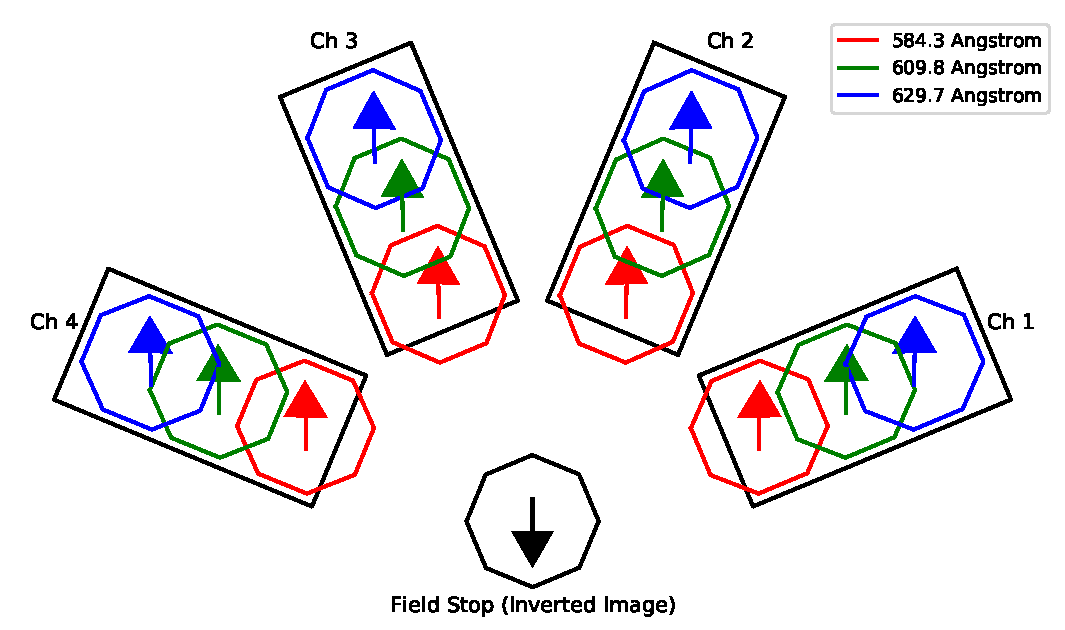
\includegraphics{detector_layout}
				\caption{A modeled layout showing the orientation of each ESIS channels' detector relative to the solar image at the octagonal fieldstop.  The locations of the brightest wavelengths (\hei, \mgxbright, and \ov) in the passband are shown on each detector.  The \hei \ line  extends off the detector edge by design, as can be seen in Figure \ref{fig:L0_to_L1}. }
				\label{fig:level_1_array}
			\end{center}
		\end{figure}

    	Each grating and detector pair, referred to as a channel in this paper,
    	is itself an independent slitless imaging spectrograph.  
    	The channels are arrayed at $45^{\circ}$ increments about the axis of symmetry of the paraboloidal primary mirror such that each channel disperses the solar image a different direction. 
    	Hence, each of these channels capture a unique projection of the spatial spectral cube, shown in Figure \ref{fig:level_1_array}. 
    	As shown, each channel captures the Sun imaged through the octagon and dispersed at different relative angles with respect to solar north. Combining these four channels creates a CTIS. 
    	Exposures from all four channels are gathered nearly simultaneously by triggering the frame transfer in three of the cameras by a single ``master'' camera. 
    	The ESIS instrument currently has 4 channels, but is built to accommodate up to 6 (limited by interference with the optical bench).

    
	\subsection{Launch and Data Collection} 
		\begin{figure}
			\begin{center}
				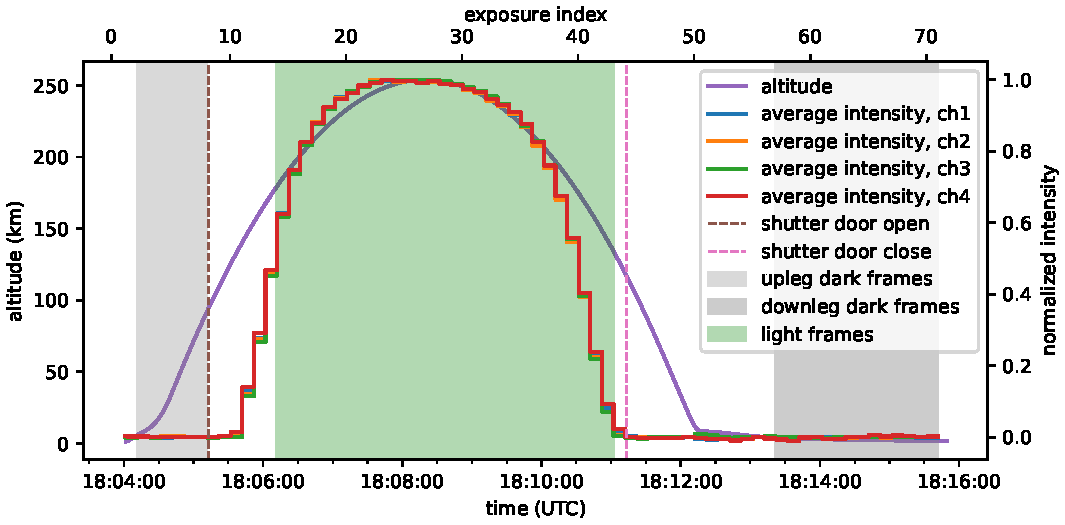
\includegraphics{signal_and_altitude_vs_time}
				\caption{The altitude of the ESIS rocket determined from White Sands Missile Range radar data as a function of elapsed time from launch.  The event times listed in Table~\ref{tab:data_info} are labeled.}
				\label{fig:timeline}
			\end{center}
		\end{figure}

		ESIS was launched at \timeMissionStart~UTC
		on \dateMission\ from White Sands Missile Range.  Figure~\ref{fig:timeline} provides the height of the sounding rocket as a function of time, determined from % White Sands Missile Range 
		radar measurements, as well as several key events during the flight.  
		The ESIS cameras began exposing at launch and continued to record full detector ($\sim$2k$\times$1k) images with a 10\,s exposure and cadence throughout the flight. Images taken while the
		experiment shutter door was closed (i.e., during the initial  boost phase of the rocket flight, and ballistic ascent to approximately 100\,km altitude) serve as darks.  
		At \timeMissionShutterOpen\ after launch, the shutter door %to the experiment 
		opened.  
		The Sun was acquired by the Solar Pointing And Rocket %and Aerobee 
		Control System (SPARCS) and the ring laser gyro (RLG) was enabled at \timeMissionRlgEnable\ indicating the rocket was in Fine Pointing Mode.  
		During this mode, SPARCS maintained a constant target; however, thermal expansion of optical components inside the instrument caused the apparent drift of the solar image on the detectors, as described in Section 3.  
		At  \timeMissionShutterClose, the shutter door closed ending solar observations. Exposures continued until the system shutdown at \timeDataStop, providing several additional dark frames at the end of the flight.   A summary of the flight and data collected is given in Table~\ref{tab:data_info}.
		
	    \dateMission\ was a very quiet day on the Sun.  
	    In fact, the last  B-class event detected by GOES \citep{GOES} prior to the ESIS launch was July 7, 2019.  Because of this exceptionally quiet period on the Sun, we chose to point at disk center. 
	    The actual pointing of the center of the ESIS octagonal field stop and roll were found after flight by comparing the ESIS exposure nearest apogee at \timeApogeeFrame\,UTC to the closest 304\,\AA \ image in time taken by the Atmospheric Imaging Assembly \citep[AIA][]{Lemen2012}, taken at \aianearapogee.  
	    The ESIS field of view projected onto the AIA 304\,\AA\ image is shown in Figure \ref{fig:fov} as a green octagon.  
	    The pointing was found to be $\approx$ \esispointing \ and the roll offset was found to be $\approx \esisroll$ \ (clockwise about Sun center), both within the tolerances for SPARCS pointing.  
	    Figure \ref{fig:fov} shows the full-disk AIA\,304\,\AA\ image. 
	    The ESIS FOV is indicated by the octagon.  
	    
		Each of the ESIS cameras collected 71 images during flight.  
		The first two images are unusable; the first image has an exposure time of 0\,s and is basically a dump of the dark current in the camera, while the second image has an exposure time slightly longer than 10\,s caused by the cameras syncing to a single trigger of the master camera.  
		All the other images have a 10\,s exposure time. 
		29 of these images were light frames, meaning the shutter door was open and the RLG was enabled. 
		The time during the rocket flight when light frames were collected is shaded green in Figure \ref{fig:timeline}.  
		Light emitted by the Sun is absorbed by the Earth's atmosphere.  
		The degree of absorption depends upon the column of the atmosphere that the telescope is looking through. The wavelength dependence of atmospheric absorption is weak, on the order of a few percent across the ESIS passband.  
		Figure~\ref{fig:timeline} shows the mean intensity in each of the ESIS channels as a function of time.  Atmospheric absorption clearly impacted the observations in the up and down legs of the flight.  
		Accounting for atmospheric absorption will be discussed in Section 3.  
		Though there are \numDataFrames\ light frames, the first and last several frames were greatly impacted by atmospheric absorption and have limited usefulness.  As the rocket was re-entering the atmosphere, a transient signal affects some of the images that would otherwise be considered darks.  It is likely due to violent deceleration when the payload encountered Earth's atmosphere.
		This effect can be seen as the small bump in the mean intensities at roughly 18:12:20 in Figure~\ref{fig:timeline}.  
		We restrict the dark frames to the data taken after the first two images, but before the shutter door opened in the upleg, and after the transient in the downleg; these times are shaded with gray in Figure~\ref{fig:timeline}.  
		In total there were \numDarkFrames\ usable dark images.  
		
		
		
		\begin{figure}
			\begin{center}
				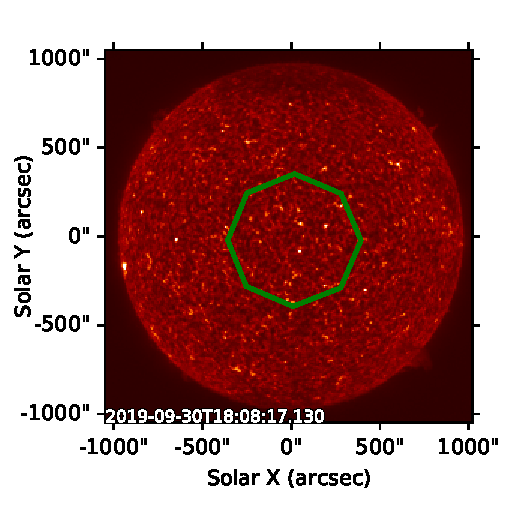
\includegraphics{esis_pointing}
				\caption{The reference AIA 304\,\AA\ data taken at \aianearapogee \ was used for determining the absolute pointing. The octagon indicates the ESIS FOV.}
				\label{fig:fov}
			\end{center}
		\end{figure}
	

		\begin{table}
		\begin{center}
			\caption{ESIS Flight Data Summary}
			\label{tab:data_info}
			\begin{tabular}{ll|ll}\hline
				Launch Date & \dateMission & Image Size  & \imageShape~pix\\
				Data Acquisition Time & \timeDataStart--\timeDataStop~UTC & Avg. Noise: & \readoutNoise\\ 
			    Pointing   &  $\approx$ \esispointing & Avg. Gain &   \gain \\
				Field of View  & $\approx$ \esisfov octagonal  & Exposure Time & 10\,s \\
				Roll & $\approx$ \esisroll CW & No. Light Exp: &\numDataFrames\\
			    Spatial  Plate Scale  &  \plateScale & No. Dark Exp: &\numDarkFrames \\
				Spectral  Plate Scale  &  \dispersion & \\
					\hline
			\end{tabular}
		Analog-Digital Unit (adu)
		\end{center}
		\end{table}
		
		



	
\section{Data} 

We have established several levels of data processing that are described in detail below.
Level 0 represents the raw data that was obtained by the four different cameras during flight.
Level 1 data incorporates %prepares raw CCD data for scientific work through 
a quadrant dependent bias and gain correction, cropping of non-active pixels, and dark subtraction.
Normally, for solar observatories like AIA, higher level data would be further corrected for solar pointing and roll by interpolating the data onto a common grid, referenced to solar coordinates.\footnote{See the Guide to SDO Data Analysis, \url{http://helio.cfa.harvard.edu/trace/SSXG/ynsu/Ji/SDO_Data_Analysis_guide.pdf}.}  For ESIS this step would be complicated, and would not be the best treatment of the data.  
First, the spatial-spectral overlap on the detector complicates the notion of image alignment. Second, interpolation inherent in such geometrical corrections degrades spatial resolution unnecessarily.  
Finally, the ESIS optics slightly distort the solar image, mainly due to the tilt of each CCD and also anamorphic magnification by the gratings, which occurs along the dispersion direction for each channel. 
In fact, the relationship between position and wavelength in each pixel depends on distortion parameters which we expect to vary subtly across the field of view, so that the distortion cannot be undone without simultaneously inverting the spatial-spectral cube across all wavelengths.
Because of this complication, we define two additional data levels.  

Level 2 data will include updated header information with accurate coefficients of a non-linear and wavelength dependent coordinate mapping from solar coordinates and wavelength to each detector for each image. 
Each image will also be corrected for differing levels of absorption from the earth's atmosphere during the course of the flight and contain a header keyword tracking the correction as a function of time for use in instrument noise models.
In addition, Level 2 data will be despiked, and store a mask for future respiking.
Level 2 data is a necessary step toward inverted data products that cover the full ESIS wavelength range. The Level 2 distortion model must incorporate not only the optical design parameters, but the consequences of small element-by-element misalignments that inevitably occur when an optical system is built up.  This model is in active development, hence the Level 2 product will not be described further here.


In lieu of a complete Level 2 product we seek a shortcut to interpretation of the ESIS data, which  we will refer to as Level 3.
Level 3 data is comprised of a single spectral line cropped from Level 1 data and mapped to the sky plane via a non-linear coordinate transform derived from a coalignment to co-temporal AIA data and an internal coalignment of each ESIS channel to a reference channel. Over the short wavelength range corresponding to a single spectral line (for our present purpose, we will choose \ov), it is quite straightforward to characterize the distortion by comparing the ESIS data to co-temporal AIA 304\,\AA\ data. This shortcut allows us to take differences between images and perform simplified inversions that are nevertheless rich in physical detail.

The highest level data product we envision providing in the future, Level 4, is the spatial-spectral data cube, i.e., the intensity as a function of $[x, y , \lambda]$, which will be the results of various inversion methods.    
Since inversions generally do not produce unique solutions, there may be multiple Level 4 products obtained by different inversion methods.
   

The Level 0, 1, and 3 data products are described in detail in the remainder of this section. 


    
\subsection{Level 0 Data}
    
Level 0 data is the raw data collected during the ESIS rocket flight.  
Each image was written to a fits files with on-board timestamp, camera number, and other parameters, such as the read out from temperature sensors included in the header.   

Each camera includes a detector with 2048 columns and 2064 rows.  The detector is operated in frame transfer mode, meaning the exposed portion of the detector is shifted into a storage portion that is read out during the next exposure. The storage portion is simply a mechanically masked region of the detector. The intention was that the storage region would be 520 rows per quadrant while the exposed region would be 512 rows per quadrant, producing an image that was 1024 rows in total.  An oversight during implementation inverted the size of the storage and exposed region, meaning the final image had 1040 rows.  Having a larger exposed region than storage region implies that eight rows originally exposed at the central portion of the detector were not behind the mechanical mask when the read out was initiated. However, because these rows were only unmasked for roughly 20\,ms, as compared to the 10\,s exposure time, there was no discernible impact on the data. 



The data is read out through 4 ports, corresponding to the four quadrants of the detector.  The read out register has 50 additional dummy pixels, or non-active pixels (NAPs), that are read out before each row of the detector data.  When the detector is read out, those 50 pixels are stored as part of the image.  Two additional ``overscan'' pixels are read after each row of data and also stored as part of the image.  A stored Level-0 data file, then, is 2152$\times$1040 pixels.   During pre-flight lab testing, it was found that the median intensity in columns 21-50 of the NAPs of each read out port are an excellent proxy for the detector bias.  Additionally the data from each port is converted from analog to digital through a unique circuit.  Though the same components were used, slight variations in the circuits caused slight differences in the gain (elec / DN) and read  noise associated with each quadrant.  The gain for each quadrant in each camera was measured prior to flight.  The noise was measured from usable dark images during flight.  The average and standard deviations in these values are given in Table~\ref{tab:data_info}.
    
\subsection{Level 1 Data}
	    \begin{figure}
	    	\centering
	    	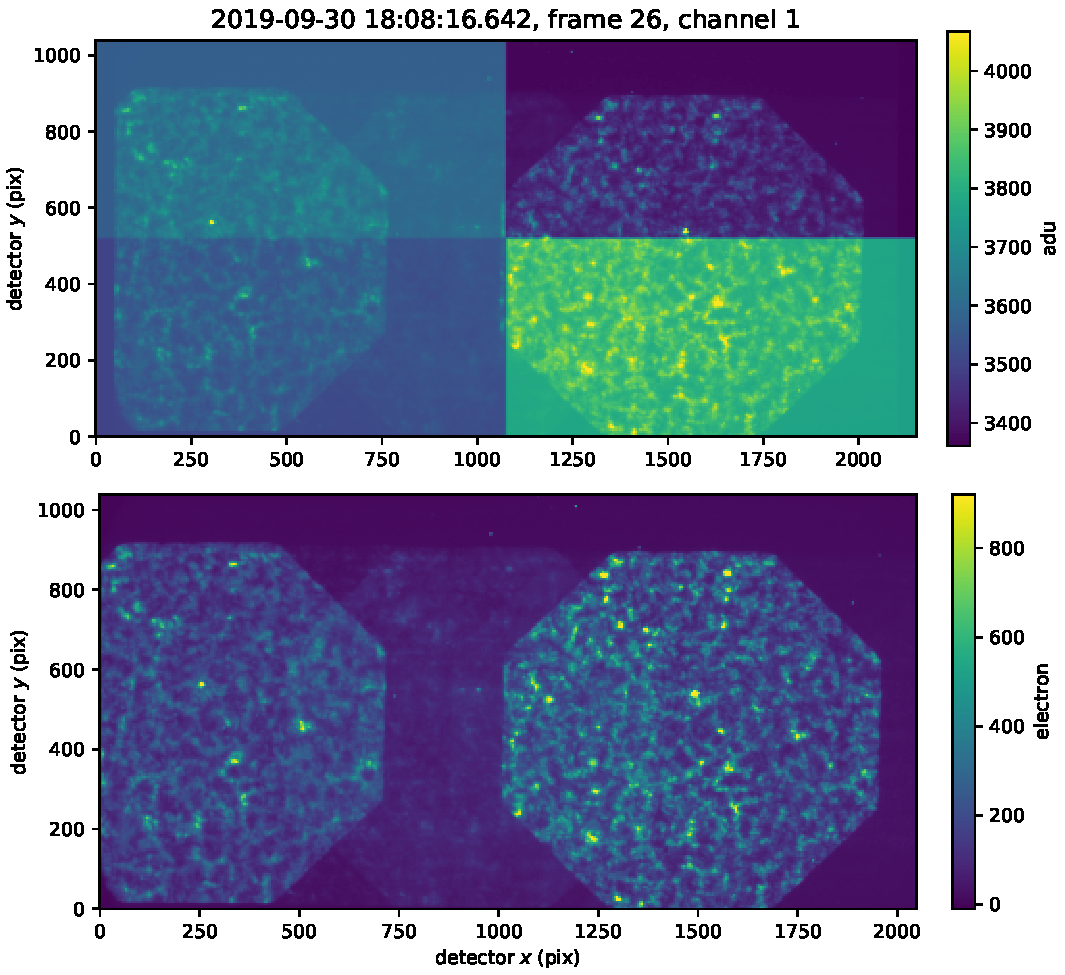
\includegraphics{L0_to_L1}
	    	\caption{The top panel is the raw, Level 0 image captured by Channel \defaultChannel\ of ESIS during apogee. The bottom panel is the same image after Level 1 processing. The Sun viewed through the octagonal field stop in the \ov \ spectral line is on the right side of the detector, this portion of the detector was cropped to generate Level 3 data.  The Sun viewed through the octagonal field stop in the \hei \ line is partially on the left side of the detector. The \mgxbright \ line is between and partially overlapping both of these two strong lines.}
	    	\label{fig:L0_to_L1}
	    \end{figure}
    	
A summary of the flight data parameters, as described in the preceding sections, is provided in Table~\ref{tab:data_info}. 
For each channel, there were \numDataFrames\ light images that were processed into Level 1 data and \numDarkFrames\ dark images used to process the data.
Our procedure to convert from Level 0 to Level 1 is described below. An example of a Level 0 and Level 1 image is shown in Figure~\ref{fig:L0_to_L1}.

\begin{enumerate}
    \item Calculate and subtract the bias of each quadrant of each usable image (light or dark) by taking the median of columns 21-50 of the NAPs for each read out port.   
    \item Create a master dark image for each channel by taking the median along the time axis of all the bias-subtracted usable dark images.
    \item Subtract the master dark from each bias-subtracted light image.
    \item Crop each image to remove the non-active and overscan pixels.
    \item Convert images from DN to electrons by multiplying each quadrant of each image by the gain for that quadrant.
\end{enumerate}
The resulting Level 1 dataset contains each channel's image sequence in units of photoelectrons.
In addition to the images, the Level 1 fits header is updated with the time, exposure length, and altitude associated with each image using standard FITS header keywords.   
	

\subsection{Level 3 Data} \label{sec:level 3}
 
    
\newcommand{\vigfit}{[.35, 0.28, 0.34, 0.6]}
\newcommand{\levthreetime}{18:08:46}

The ESIS Level 3 data product is created to provide a co-aligned, single wavelength image in each channel for quick identification of events with significant line-of-sight velocities and easy comparison with coordinated data that does not require inversion. 
Level 3 data also allows for single wavelength inversion prior to the completion of the final optical distortion model and the Level 2 data product.  A demonstration of both qualitative and quantitative analysis of Level 3 data is given in Section 4.  

Level 3 data is generated directly from Level 1 as follows:
\begin{enumerate}
    \item Level 1 data is converted to units of photons in the target wavelength and then despiked.\label{step:photons}
    \item Optical distortion and internal co-alignment are corrected, and each channel is resampled onto an appropriately cropped common grid, with known alignment to AIA data.\label{step:distortion}
    \item Each channel is corrected for vignetting.\label{step:vignetting}
\end{enumerate}
Figure \ref{fig:coalign}a shows an example of a Level 3 image from Channel 2 taken at \levthreetime. All three steps make the assumption that the intensities are associated with the target wavelength. No attempt is made to distinguish photons of other wavelengths that may overlap with the octagonal field stop image in the target wavelength, so Level 3 is a useful construct for a target wavelength corresponding to a strong spectral line with minimal contamination. The above steps are described in greater detail below.


	\begin{figure}
		\centering
		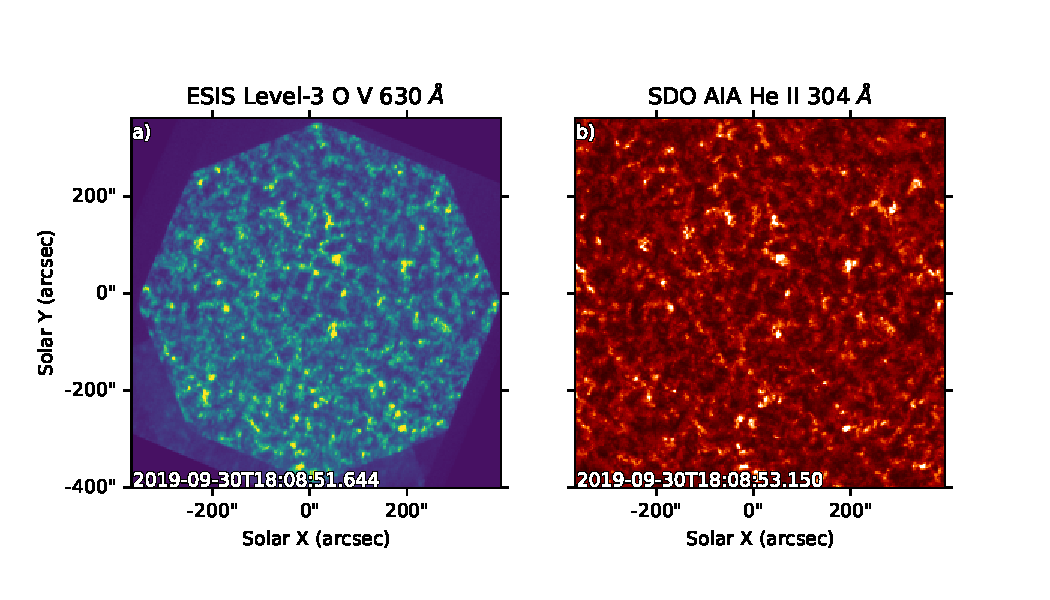
\includegraphics{aia_coalign.pdf}
		\caption{(a) An example of the Level 3 data product from Channel 1 taken at \levthreetime. This data has been aligned using nonlinear mapping parameters to the closest co-temporal AIA 304\,\AA\ image, shown in (b). }
		\label{fig:coalign}
	\end{figure}
    	
    
\subsubsection{Conversion to Photons and Despiking}
In order to use Level 3 data for early inversion the intensity needs to  converted to photons in order properly account for uncertainty in the data.
The conversion from electron to photon is done to Level 1 data prior to co-alignment efforts.
The intensity in photons, $I_{\gamma}$, then becomes
\begin{equation}
  I_{\gamma} = I_{\SI{}{\elementarycharge}} * 3.6 \frac{\SI{}{\electronvolt}}{\SI{}{\elementarycharge}} * \frac{\lambda}{hc},
\end{equation}
where $I_e$ is the Level 1 intensity in electrons, and $\lambda$ is the target wavelength.
With a Silicon band gap energy of \SI[per-mode=symbol]{3.6}{\electronvolt\per\elementarycharge}, and an energy per \ov \ photon 
of 19.6\,\SI{}{\electronvolt} gives 0.18 photons per electron.


Due to geomagnetic activity on launch day, our detectors received a substantial number of charged particle hits. 
We therefore elected to despike the data.
Available despikers were difficult to tune in such a way that they eliminated particle hits, but not small transient events (e.g. explosive events). We therefore developed a new despiking algorithm, which is identified in Appendix \ref{despike}.

        
\subsubsection{Optical Distortion Correction and Channel Co-Alignment}
   
  The four ESIS channels were spatially co-aligned in two steps.
First, each ESIS image is cropped around the \ov \ spectral line, (roughly pixels 1000 - 2048 of the Level 1 data shown in Figure~\ref{fig:L0_to_L1}) and then co-aligned to the closest AIA 304\,\AA\ image in time.  
The AIA 304 channel was chosen for co-alignment because it is the AIA EUV channel most visually similar to O V, in both the background and bright events (Figure \ref{fig:coalign}b).
Prior to co-alignment each AIA image was prepped to Level 1.5 using the aiapy routines \texttt{aiapy.calibrate.update\_pointing()} and \texttt{aiapy.calibrate.register()}.
The co-alignment was achieved through a linear coordinate transformation of the cropped ESIS image that maximizes the zero lag cross-correlation between it and AIA 304, the results of this are shown in Figure \ref{fig:coalign}.

Since ESIS has a slightly non-linear distortion function \citep{ESIS}, an additional internal alignment step is performed. 
Sub-pixel accuracy of the ESIS inter-channel alignment is critical to our tomographic inversion of the data to obtain line profiles, so we exercise more care than with the alignment to AIA.
Using a single ESIS channel as reference, in this case Channel 2, each other channel is co-aligned to it via a quadratic coordinate transformation that maximizes the zero-lag cross-correlation. 
Figure \ref{fig:cc} shows the ratio of peak cross-correlation after the quadratic internal alignment to that of the linear co-alignment with AIA for every camera pair and every exposure
A ratio greater than 1 implies this second step improved co-alignment.
We find that the internal alignment improves not only the co-alignment between each channel and the reference channel (dots in Figure \ref{fig:cc}), but also the co-alignment between every other combination of channels (stars in Figure \ref{fig:cc}).
This ratio is greater than 1 in all cases and shows a less than 1 percent improvement in peak correlation, demonstrating the subtle non-linearity of the ESIS optical distortion function.
In pixels, this corresponds to an average change in mapping of $\approx 0.4$ pixels.

After the co-alignment is complete each Level 3 image has been re-binned to AIA resolution, 0.6 arcsecond per pixel, and can be assigned the WCS information \citep{WCS} from the nearest image AIA in time, providing pointing information and easier co-alignment with coordinating instruments.



 \begin{figure}
	\centering
	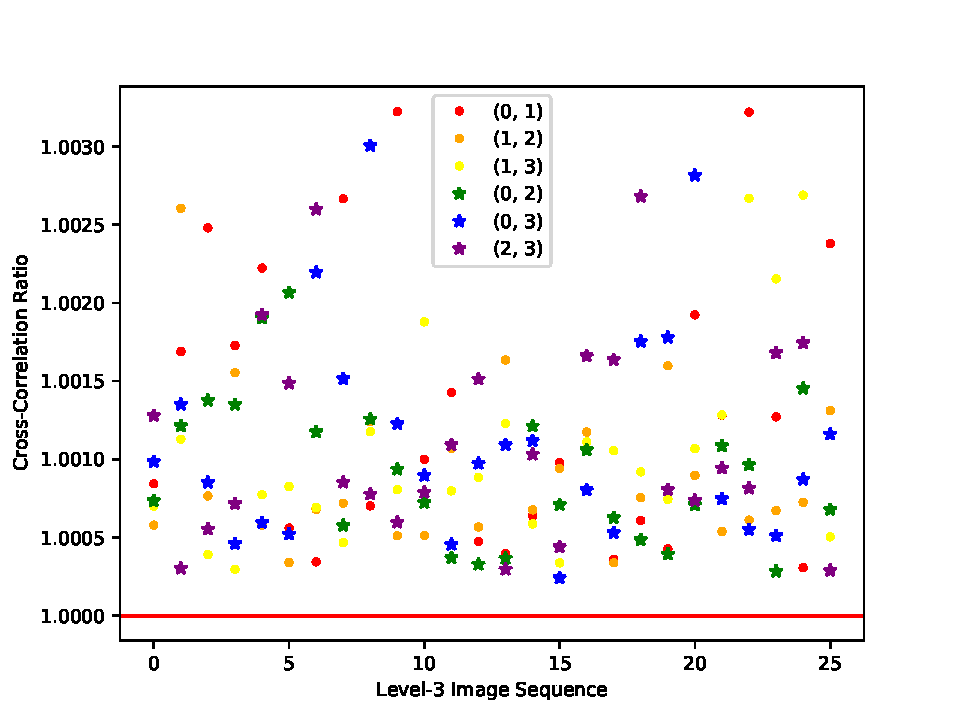
\includegraphics{internal_align.pdf}
	\caption{For each ESIS exposure (or image sequence) every channel pair, labeled in the legend, is cross-correlated to measure internal alignment quality.  The ratio of zero lag cross-correlation after a quadratic transformation to that of a linear transformation is plotted.  Every point is above the ratio = 1 line, indicating improved internal alignment for every combination of ESIS channels at each exposure.}
	\label{fig:cc}	
\end{figure}

 \begin{figure}
	\centering
	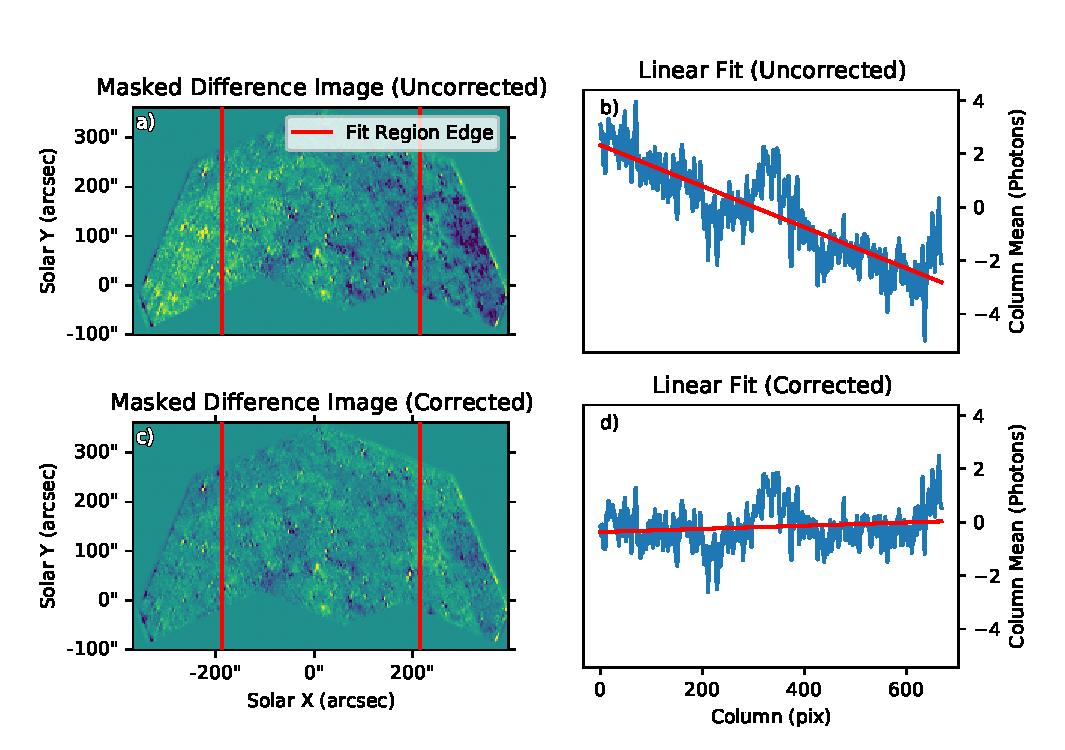
\includegraphics{vig_correct.pdf}
	\caption{Panels a and c show example difference between images with \mgxbright \ masked that are uncorrected and corrected for vignetting respectively.  The line fit to the column mean as a function of column (fit between the red bars) shows a difference in background of $\approx 5$ photons before correction (panel b) at the edges of the field of view, and .4 photons after (panel d). }
	\label{fig:vig_correct}
\end{figure}

\subsubsection{Vignetting Correction}
  
Each ESIS channel has a linear trend in intensity across the octagonal field of view along the dispersion direction due to internal vignetting in the optical system caused by having multiple stops in the optical system \citep{ESIS}.
In the co-aligned Level 3 images, where solar north is rotated to the top of the image, the dispersion axes run at different angles relative to solar north in each channel, so the impact of the vignetting field can be seen in the linearly trending background when taking the difference between two channels (Figure \ref{fig:vig_correct}a).
We corrected the vignetting by dividing out a linearly trending background, aligned to the dispersion axis, in every image. The parameters of this linear trend in each channel were obtained by minimizing the intensity trend seen in Level 3 difference images.

We define the vignetting field for the $i$th channel, at each time index, $s$, as a function of the pixels in the Level 3 data, $(x,y)$, as 
	\begin{equation}
		V_{is}(x,y) = \frac{m_i}{r_t} * [r(x,y,s) - r_0] + 1,
		\label{eqn:vignet}
	\end{equation}
where
	\begin{equation}
		r = x_0 + [\cos(\alpha_i)(x-x_0-x_{\text{drift}}*s/s_t) - \sin(\alpha_i)(y-y_0-y_{\text{drift}}*s/s_t)].
		\label{eqn:vignet2}
	\end{equation}

In Equation \ref{eqn:vignet}, $r_0$ is equal to 65 pixels, and represents the distance from the Level 3 image edge to the ESIS field stop octagon edge at $s = 0$, the first Level 3 image.
The width of the octagon along the dispersion direction, $r_t$, is equal to 1140 pixels.
In Equation \ref{eqn:vignet2},  $\alpha_i$ is the angle of rotation of each ESIS Level 3 image relative to a Level 1 image row.
In this case, $\alpha_i = [112.5^{\circ}, 67.5^{\circ}, 22.5^{\circ}, -22.5^{\circ}]$ for Channels 1-4, respectively.
The vignetting field is rotated about the point $[x_0, y_0] = [635,635]$, which is the nominal center of the Level 3 image, to account for the change in dispersion direction.
ESIS Level 3 images have a fixed solar coordinate, therefore the the field of view defined by the octagon drifts as a function of time index, $s$, due to a slight pointing drift during the flight. 
The empirical drifts are $[x_{\text{drift}},y_{\text{drift}}] = [8, -4]$ pixels. 
The total number of Level 3 exposures is $s_t=29$. 


In the above relations, we have just four free parameters, the slopes $m_i$. 
The four channels of ESIS give 6 possible difference images for fitting the vignetting function for each image sequence $s$. 
When the average slope of all 174 combinations (6 difference images per each of the \numDataFrames \ exposures) is minimized we consider the vignetting corrected.

Measuring the trend from the data is additionally complicated by the overlap of the bright \mgxbright \ line.  
This line overlaps different regions of the field of view in each channel, see Figure~\ref{fig:mgx_overlap}.  
Therefore when fitting the background we restrict ourselves to the portion of the field of view without the \mgxbright \ overlap in any channel.
We also only use column means between the red bars in Figure \ref{fig:vig_correct} to ensure sufficient pixel numbers in each column.  

The resulting final fit, $m_i = \vigfit$, differs from the field predicted using ray tracing and geometric optical models \citep{ESIS}, which can be attributed to a few likely culprits. 
% One source of error likely comes from the imprint of adjacent spectral lines, the most obvious being that of \mgxdim \ visible in Figure \ref{fig:vig_correct}c.
% Since this Mg {\sc x} line overlaps almost entirely with O {\sc v}, and has an identical vignetting function, it adds intensity that prevents a perfect fit. 
% If this were the only source of discrepancy between the vignetting function predicted by the raytrace and the fits obtained from the data, then we would simply use the same, predicted vignetting for every channel. 
% However, we can anticipate slightly different vignetting in each channel due to variations in assembly so we allow each channels slope to vary independently.
% A misalignment of the ESIS field stop center, the ESIS primary optic center, and the center of the ESIS grating array, all shift the geometry of the ESIS central obscuration and can easily modify the vignetting field in each channel.
% Despite the uncertainties in vignetting, which we have found difficult to quantify, Level 3 differences are much flatter in intensity post vignetting correction as is seen in Figure \ref{fig:vig_correct}c, and will therefore lead to a higher fidelity intensity recovery when inverting Level 3 data.
% The resulting final fit, $m_i = \vigfit$, differs from the field predicted using ray tracing and geometric optical models \citep{ESIS}, which can be attributed to a few likely culprits. 
Our optical models assume a perfectly built and aligned ESIS instrument, resulting in each channel having identical vignetting.
A misalignment of the ESIS field stop center, the ESIS primary optic center, and the center of the ESIS grating array, all shift the geometry of the ESIS central obscuration and can easily modify the vignetting field in each channel.
% This misalignment would result in each channel having a vignetting field with a different slope.
When performing this vignetting correction we found we needed to allow the slope to vary for each channel to achieve a quality fit.
Another difference between the fit and the model is the slope of each vignetting field.
Our fits to Level 3 data show less vignetting in every channel than is predicted by our optical models. 
This likely comes from the imprint of adjacent spectral lines, the most obvious being that of \mgxdim \ visible in Figure \ref{fig:vig_correct}c.
Since this Mg {\sc x} line overlaps almost entirely with O {\sc v}, and has an identical vignetting function, it adds intensity that prevents a perfect fit. 
It is also possible that there is a subtlty to the ESIS vignetting calculation that we have failed to account for in our ray trace and geometric optical models.
Despite the uncertainties in vignetting, which we have found difficult to quantify, Level 3 differences are much flatter in intensity post vignetting correction as is seen in Figure \ref{fig:vig_correct}c, and will therefore lead to a higher fidelity intensity recovery when inverting Level 3 data.

  
        
        \begin{figure}
        	\centering
        	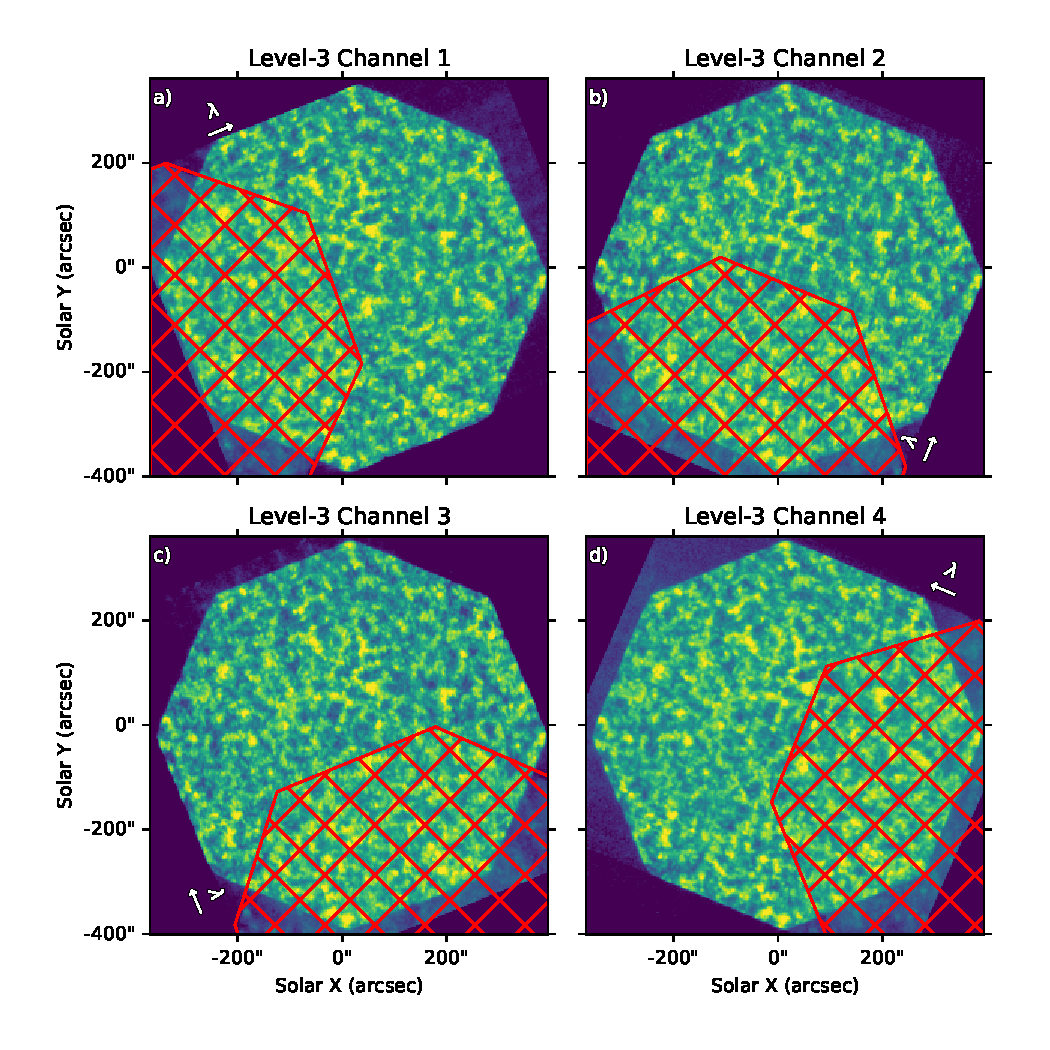
\includegraphics{mgx_overlap.pdf}
        	\caption{The red hashed region shows the overlap of the \mgxbright \ spectral line in each channel that is masked prior to the vignetting correction and intensity normalization. These images are displayed in log scale in an attempt to bring out the subtle contamination.  The outline of the Mg\,{\sc x} can be seen very clearly in difference images like Figure \ref{fig:l3_dif}. }

        	\label{fig:mgx_overlap}
        \end{figure}
        
        

        
    \subsubsection{Relative Radiometric Correction }
        The intensity of each channel is normalized by by equalizing the image mean over the least contaminated shared piece of Sun, and is therefore performed after inter-channel co-alignment and the vignetting correction.
        We divide each image by its mean in the region of the field of view uncontaminated by \mgxbright \ in every channel (shape shown in Figure \ref{fig:vig_correct} a and c) and multiplying it by the mean in that same region from the brightest image in the brightest channel (Channel 2 at apogee)
        This not only normalizes the intensity between each channel at every exposure, but also corrects for the effects of atmospheric absorption mentioned in earlier sections. 


\section{Preliminary Results}
 
	   In this section, we provide a preliminary analysis of the ESIS Level 3 data. Our aims are to assess the ability of the ESIS data to (1) provide velocity signatures of dynamic events and (2) aid in developing a useful qualitative and quantitative understanding of the events.
	   Despite the lack of solar activity, ESIS managed to capture tens of small, transient events and one larger event during the $\approx 5$ minutes of observation in the \ov \ spectral line.  
	   We analyze five example events in this section.  
	   
    \subsection{Level 3 Difference Images} \label{sec:dif_images} 
    	Early work with MOSES images demonstrated the utility of examining differences between different projections of the spatial-spectral cube (channels) to identify solar features with significant line-of-sight velocity \citep{Fox2010,Fox2011,Rust2017,Rust2019}, and to diagnose spectral contamination \citep{Rust2017, Rust2019}.
    	It is for this reason that we developed a Level 3 data product, spatially co-aligned in O\,\textsc{v}, %quickly 
    	that would allow us to take differences between ESIS channels.
    	Each ESIS channel disperses solar features in a different direction relative to solar north, determined by the orientation of each grating.
    	The positive dispersion direction in each Level 3 image is indicated by the arrows  in Figure \ref{fig:mgx_overlap}.
    	%In the case of an eruptive event with a velocity signature, the Doppler shifted intensity 
    	
    	Figure~\ref{fig:l3_dif} (and associated animation) shows the difference between Channels 2 and 3 for the full ESIS field of view.  
    	Since wavelength is dispersed a different direction in each channel, taking the difference between two
    	simultaneous, spatially aligned channels cancels the intensity in the O\,\textsc{v} spectral line core. 
    	What remains are signatures of Doppler shifts, line broadenings, and other spectral lines.
    	Before we describe signatures of Doppler shift, it may be helpful to point out certain large-scale features that arise from spectral contamination.
    	The % white 
    	yellow octagon that overlays the lower left quadrant of the image is the \mgxbright \ line that overlaps the \ov \ line in Channel 2. Similarly, a dark octagon on the lower right quadrant is the portion of the \mgxbright \ line that overlaps the \ov \ line in Channel 3.
    	
    	
    	%leaves only intensity away from the O\,\textsc{v} spectral line core.  
    	%To put it another way, subtracting the data from two channels removes all the spatial structures that overlap in the two channels and leaves  easily identifiable velocity signatures. 
    	%For our initial analysis, we focus on the dominant O {\sc v} 629.7 \AA \ spectral line in the ESIS passband. \amy{I think this is a given since it is the only one in level3}
    	In the difference image, small-scale black and white lobes frequently appear near the locations of bright features on the Sun. A few of such features are marked with red boxes and will be discussed in detail below.  
    	The small black lobes tend to lie at an angle of $-22.5^\circ$ with respect to solar north, which is the direction of dispersion of Channel 3, while white lobes tend to lie at an angle of $+22.5^\circ$ with solar north, which is the direction of dispersion of Channel 2. A sufficiently compact and well-isolated brightening functions as its own spectrograph slit. 
    	The lobes then form V-, $\Lambda$-, or X-shaped features. 
    	Furthermore, intersection of the lobes occurs at the line center. 
    	Lobes above that intersection (i.e., along the dispersion direction in both channels) indicate a red shift (V). 
    	Lobes below line center similarly indicate a blue shift ($\Lambda$). The complete X-shape indicates a line broadening in which both red and blue shifts are present.
    	
    	Although the ESIS geometry differs significantly from MOSES, which had three images taken at spectral orders $m=-1, 0, 1$
    	of a single grating, analogous Doppler signatures appeared in MOSES data. These Doppler signatures were analyzed in great detail by \citet{Rust2019}, who sliced through small events along the dispersion direction to measure \heii \ line profiles from MOSES data.
    	% Every X or V-shaped features in an ESIS difference image, Figure~\ref{fig:l3_dif}, that have obvious, and nearby, positive and negative portions indicate solar events with significant line-of-sight (LOS) Doppler velocity.   
    	% Other things to 
    	    
   		
  		\begin{figure*}
  			\centering
  			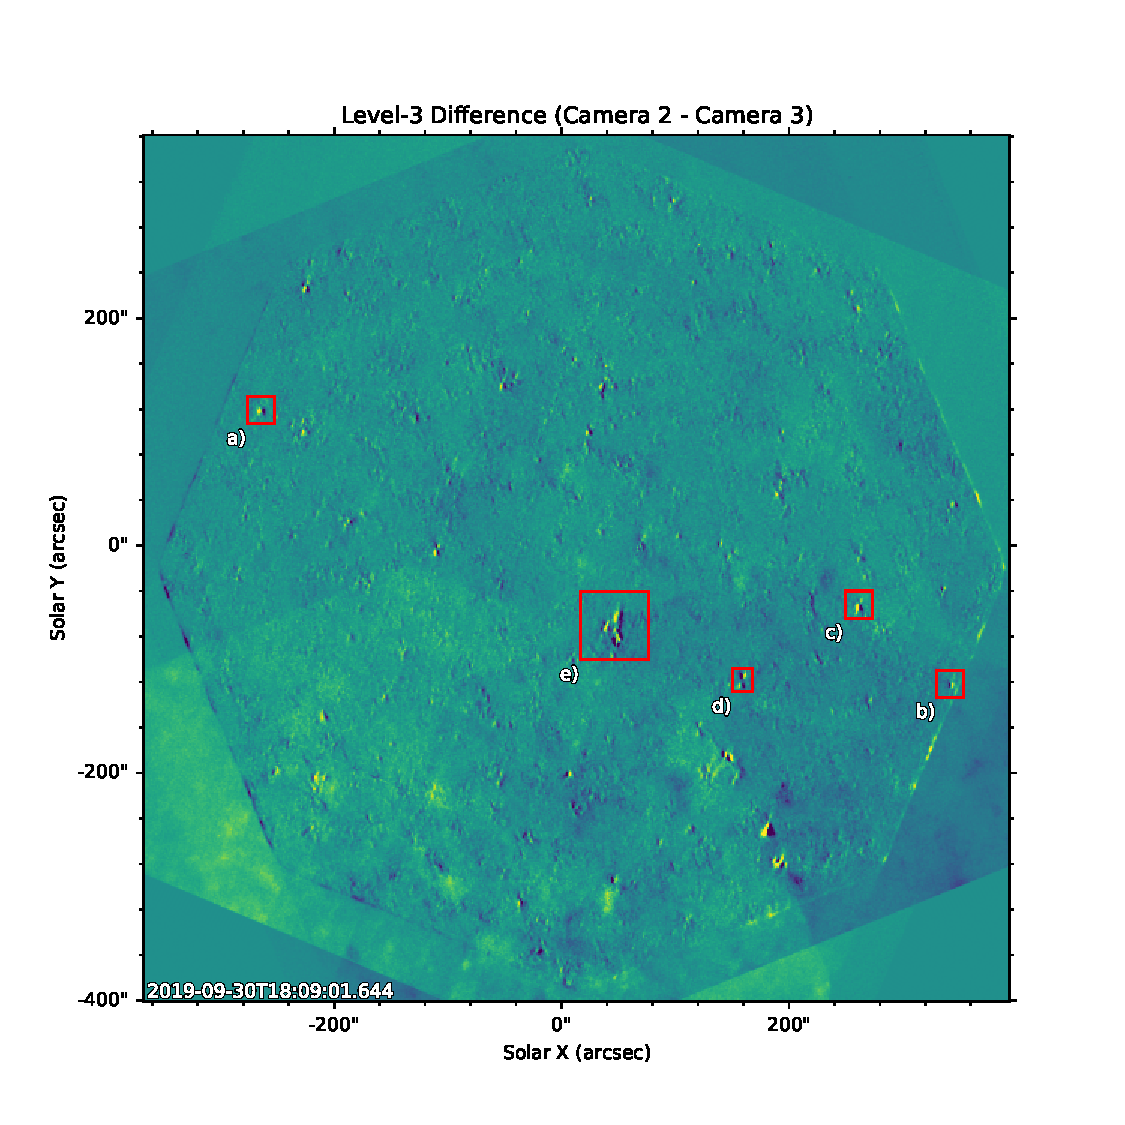
\includegraphics{l3_dif}
  			\caption{Full FOV Difference between Channel 2 and Channel 3 Level 3 images.  
  			Arrows denote the positive dispersion direction in Channel 2 and 3.
  			Events a-c are highlighted in Figure \ref{fig:dif_events}.    
  			Inverted results for Events c and d are shown in Section \ref{sec:inversions}. 
  			A time series of Event e is shown in Figure~\ref{fig:main_event}.
  			The associated animation shows these difference images throughout the ESIS observation.}
  			\label{fig:l3_dif}
  		\end{figure*}
   	
   	
 		\begin{figure}
  			\centering
  			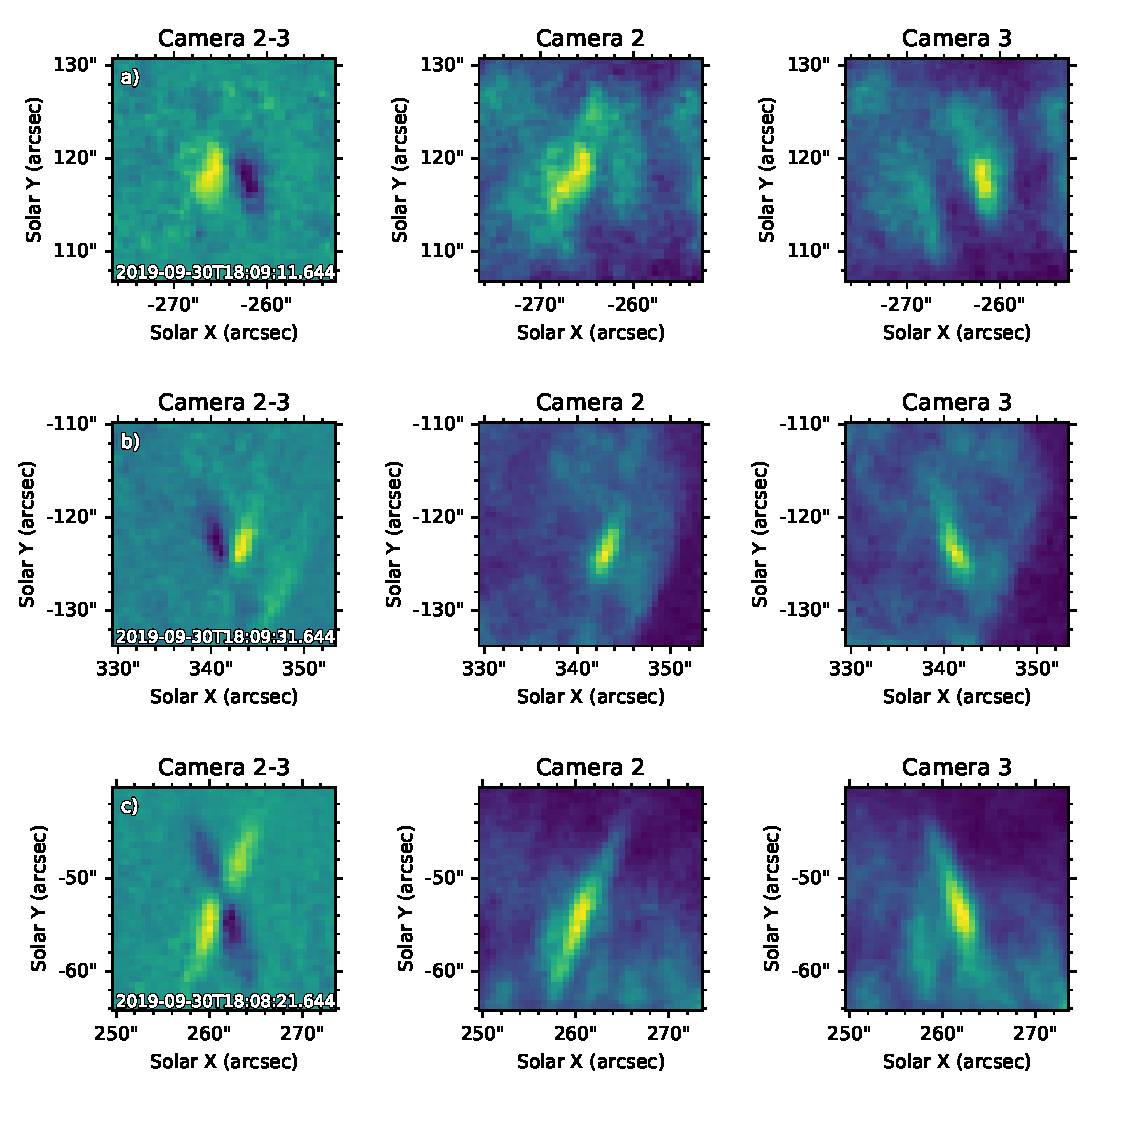
\includegraphics{dif_events}
  			\caption{Events a, b and c identified in Figure \ref{fig:l3_dif} are examples of a mostly blue, red, and broadened event, respectively. The difference between Channels 2 and 3 is shown in the left hand column, while the Channel 2 and Channel 3 intensities are shown in the middle and right columns.  The velocity signature is most easily seen in the difference image, while the straight intensities provide information on the line core intensities. 
  			}
  			\label{fig:dif_events}. 
  		\end{figure}

    	%Simple, point-like, transient brightenings with little or no spatial structure are the easiest events to interpret because their naturally confined spatial extent acts similarly to a spectrographic slit.
    	%For that reason any stretching along the dispersion direction in an ESIS image can be interpreted directly as velocity. 
    	%In these simple events, a qualitative understanding of their velocity can be ``read off'' of each ESIS difference image.
    	%This effect was explored in great detail by \citet{Rust2019}, who sliced through small events along the dispersion direction to measure \heii \ line profiles from MOSES data.
    	
    	Three features, labeled a, b, and c in figure \ref{fig:l3_dif}, serve to illustrate the $\Lambda$, V, and X morphologies described above.
    	% Here we explore the velocity signature in three examples of simple point-line events marked a-c in Figure~\ref{fig:l3_dif}.  
    	Figure \ref{fig:dif_events} shows the difference image in the first column for all three events, then the Channels 2 and 3 data in the subsequent columns. 
    	Figure \ref{fig:dif_events}a shows a $\Lambda$-shaped event with lobes pointed downward in the difference between the Channel 2 and Channel 3 Level 3 image.
    	Since we know that the direction of positive wavelength dispersion is up and to the right in Channel 2 and up and to the left in Channel 3 (Figure \ref{fig:mgx_overlap}) we immediately know that this event is predominantly blue shifted.  
    	Similarly, an upward facing V-shaped event, like the one shown in Figure \ref{fig:dif_events}b, is predominantly red shifted.
    	X-shaped events, shown in Figure \ref{fig:dif_events}c, suggest enhanced emission in both the red and blue wing of the line profile. 
    	Difference images can provide immediate qualitative understanding of these simple, point-like events.  
    	During the 5 minute rocket flight, tens of similar events were detected in the ESIS field of view.  
    	We observe that the X-shaped events are especially common in this dataset, though multiple examples of each 
    	type are apparent.
    	
    	%While this gives us a quick and qualitative understanding of a simple event, even the smallest amount of spatial extent in a given feature leads to an entanglement of spatial and spectral information making it very difficult to derive qualitative velocities without inversion. 
    	
    	\begin{figure}
    		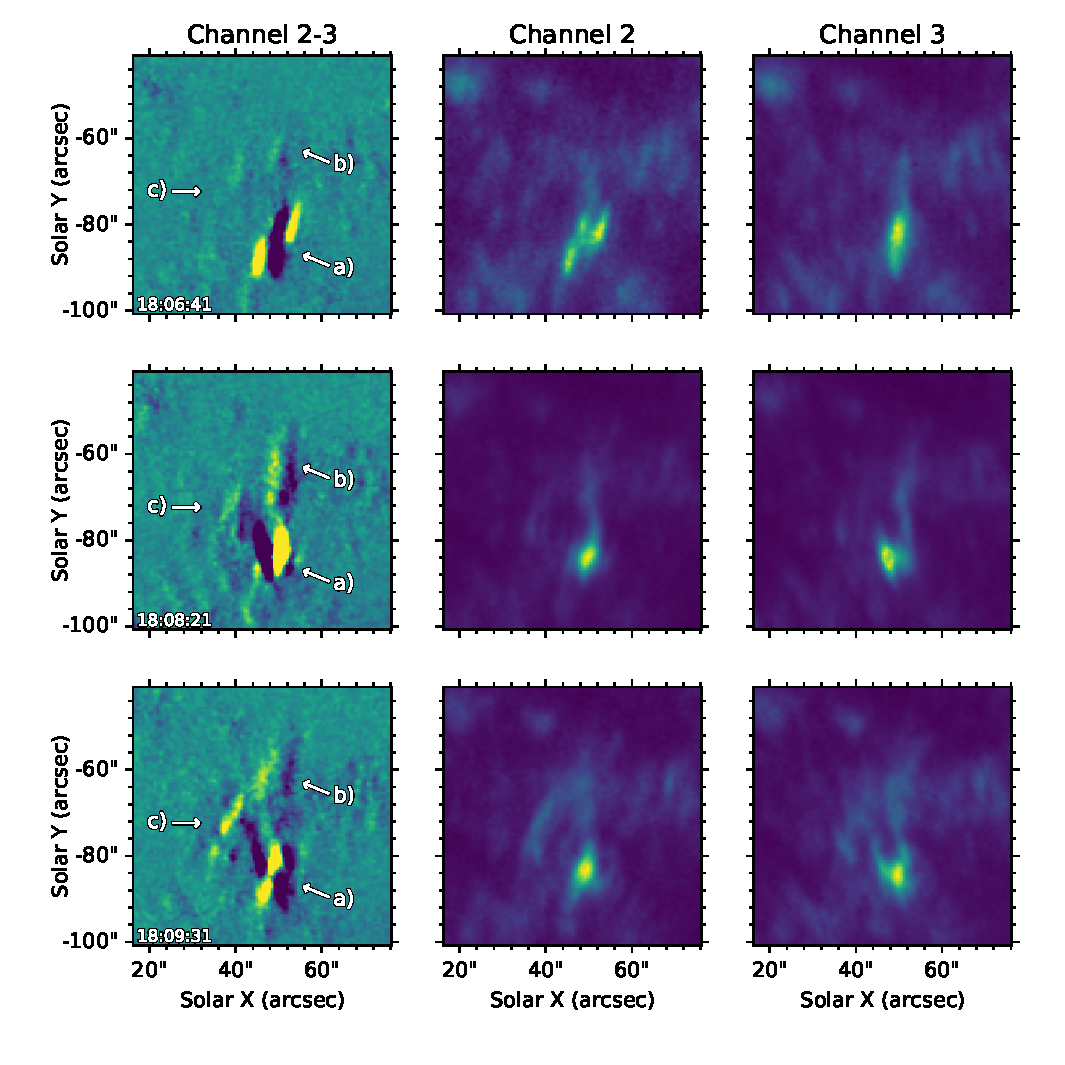
\includegraphics{main_event_dif}
    		\centering
    		\caption{The largest and most complex velocity event (e) %eruption
    		captured by ESIS shown at three different times (complete evolution in animation). The event starts as two jets (one red, one blue) with slight spatial separation, evolves into a strong red shift where the event begins paired with faint blue shifted material above, and ends in a complicated combination of velocity not easily interpreted from difference images. Co-temporal images from AIA 304\,\AA, 171\,\AA, and 193\,\AA\ are included in the animation for additional context.}
    		\label{fig:main_event}
    	\end{figure}
    
   		\begin{figure}
    		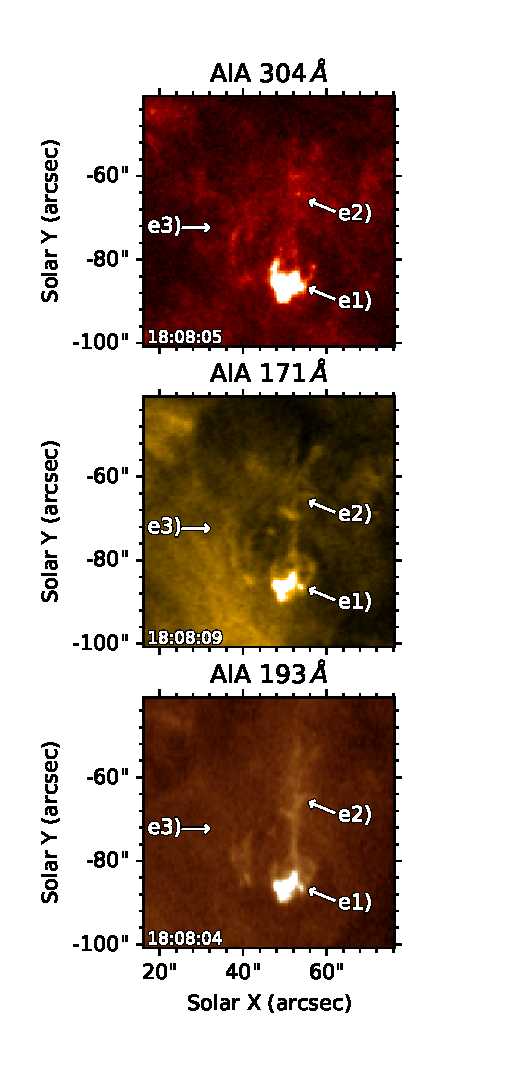
\includegraphics{main_event_aia_context}
    		\centering
    		\caption{Co-aligned AIA 304\,\AA, 171\,\AA, and 193\,\AA\ images of event e  (highlighted in Figure \ref{fig:main_event}) are shown with identical locations labeled. The location of peak intensity (e1) in the ESIS Level 3 data is also the location of brightest intensity in these EUV channels. We also note a jet like structure which is very diffuse in the cooler 304\,\AA\ images, and visible as a thin line of intensity in 171\,\AA \ and 193\,\AA \ between the e1 and e2 labels that matches the location of the faint blue shifted structure visible in Level 3 difference images. Animations of these AIA channels, included with Figure \ref{fig:main_event}, show material traveling along this line and being ejected away from location e1.}
    		\label{fig:main_event_aia}
    	\end{figure}
		
    	During the ESIS flight, we also captured a handful of spatially extended Doppler signatures that are more difficult to interpret.
    	The most obvious of these is an eruption near disk center, Event e in Figure \ref{fig:l3_dif}.
    	This large event is shown at three times in Figure \ref{fig:main_event}.
    	The entanglement of spatial and spectral information in this relatively complex event makes it difficult to derive a qualitative interpretation from the difference images (left column of the figure).
    	A cluster of overlapping positive and negative lobes in the brightest portion of the event (location e1) sometimes present as a $\Lambda$, V, or X shape, but not always, and evolve significantly in time.
    	The top row shows this event early in its evolution. 
    	Intensity is concentrated to a small region and presents as two jets, one red and one blue, with the red shifted source slightly to the right of the blue shifted source. 
    	100 seconds later (middle row), the event is dominated by a significant red shift (upward facing V) at the location of initial brightening. 
    	There is also an imprint of fainter differences above the brightest knot of intensity (location e2) showing motion along a spatially extended structure.
    	The difference lobes in this faint structure are opposite in polarity to the intensity below, and therefore appear to represent  blue shifted material ejected from the site of initial brightening.
    	This is supported by the appearance of a thin string of ejected material at the same location in AIA 304\,\AA, 171\,\AA, and 193\,\AA \ (Figure \ref{fig:main_event_aia} and the animation associated with Figure \ref{fig:main_event}).
    	By the end of the event (another 70 seconds later, bottom row) the dominant red shift subsides, leaving a complicated spectral signature at the brightest portion of the event, and in the adjacent region up and to the left (location e3).  
    	
    	So far, we have been exploiting two of the four ESIS channels with our difference image. This approach is qualitative,
    	and its limitations become apparent with complex and spatially extended dynamics as we saw in event e.
    	An understanding of ESIS difference images provides a starting point,
    	and offers a sanity check when interpreting numerical inversions that take advantage of all four projections.
    	In the following section we will focus on inverting two smaller events (c and d), and will save a more in depth analysis of Event e for a future publication. 
    	
    
    
    \subsection{Early Inversions} \label{sec:inversions}
    	In order to better disentangle the spectral and spatial information captured by ESIS, and to provide quantitative velocity information, all four channels must be combined and ``inverted'' to return a single, spatial-spectral cube, $I(x,y,\lambda)$, at every exposure.
    	For our preliminary inversions of the \ov \  ESIS Level 3 data we used a Multiplicative Algebraic Reconstruction Technique (MART).
    	MART is attractive for our first inversions because it is fast, requires no training or explicit assumptions about the data, and automatically enforces image  positivity.
    	We describe our MART implementation in Appendix \ref{MART}.
    	
    	When constructing the ESIS Level 3 data, each channel is co-aligned to a reference channel (Section \ref{sec:level 3}).
    	By doing this, we are assuming that the mean velocity in \ov \ is zero prior to inverting.
    	Work by \citet{Peter1999} suggests that the transition from a mean red shift to a mean blue shift at disk center occurs around .5\,MK.
    	Therefore, since \ov \ is a relatively hot transition region line, and is formed near .22\,MK, we expect a systematic error in our inverted velocities of less than 10\,km\,s$^{-1}$ as a result of this assumption.
    	 
    	
    	\begin{figure}
%    		IF Thesis
			\resizebox{6in}{!}{% 			
				\begin{tikzpicture}	
				%begin by adding a node for each figure
				\node[inner sep=0pt] (imgs) at (0,0)
				{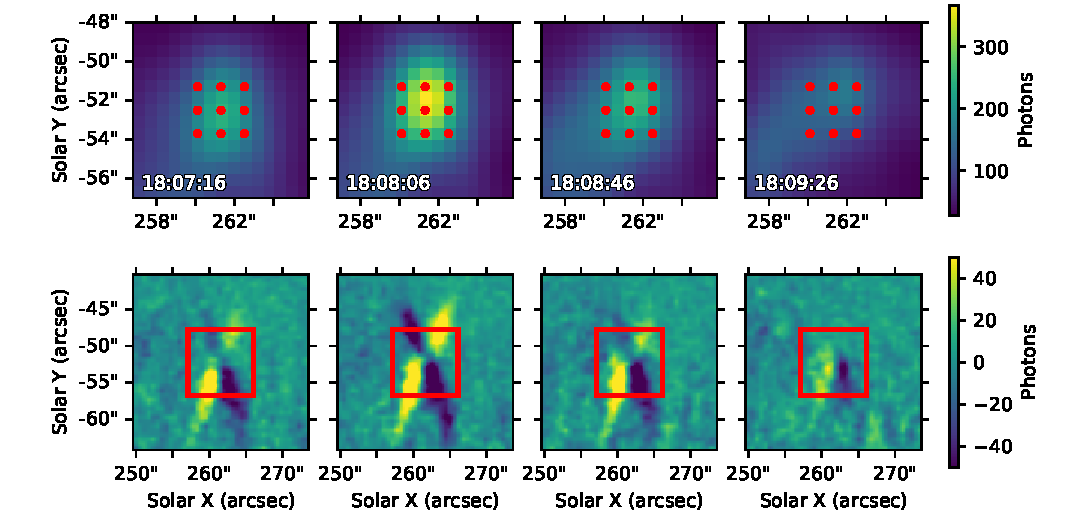
\includegraphics[]{perfectx_inverta}};
				\node[inner sep=0pt] (lps) at (0,-10.5)
				{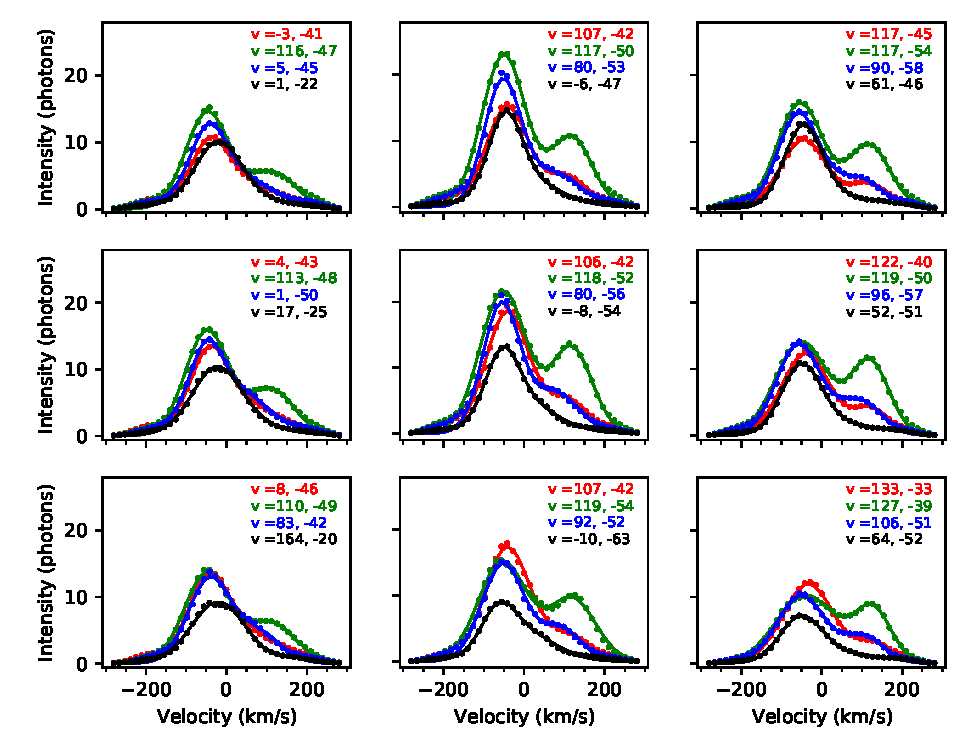
\includegraphics[]{perfectx_invertb}};
				\end{tikzpicture}
    		}
%  			\begin{tikzpicture}	
%	    		%begin by adding a node for each figure
%	    		\node[inner sep=0pt] (imgs) at (0,0)
%	    		{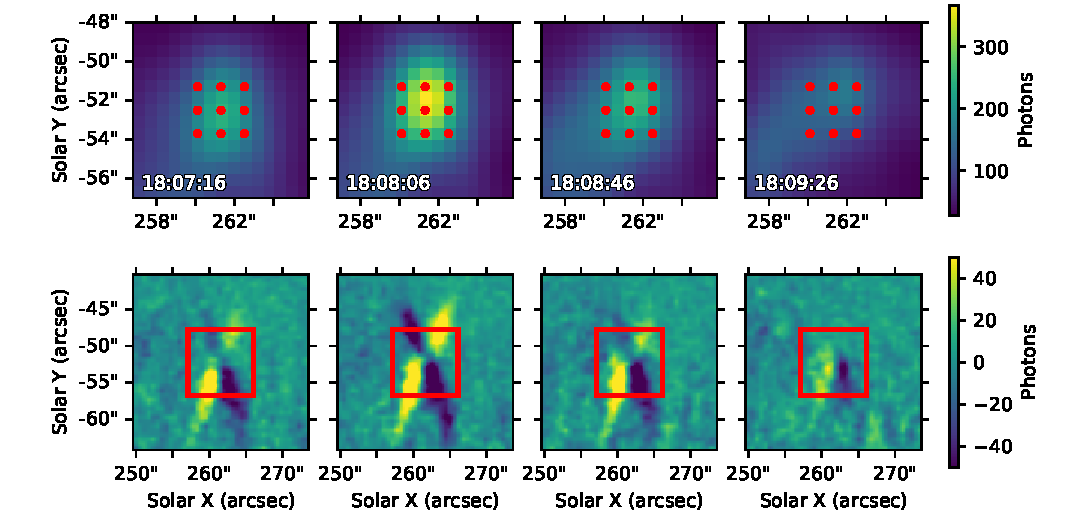
\includegraphics[]{perfectx_inverta}};
%	    		\node[inner sep=0pt] (lps) at (0,-10.5)
%	    		{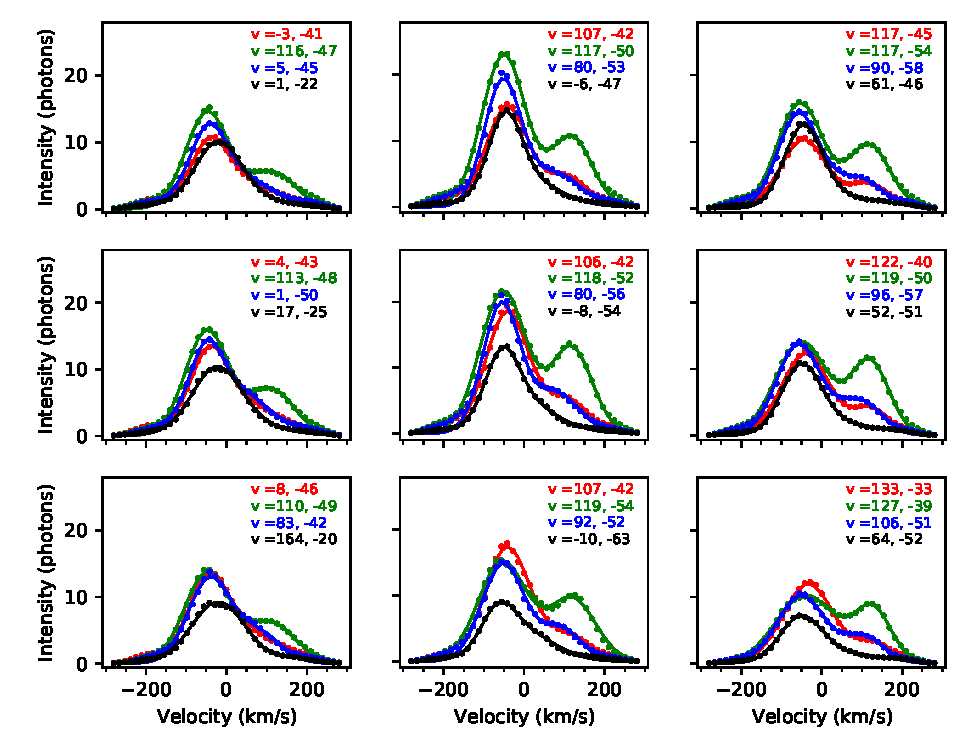
\includegraphics[]{perfectx_invertb}};
%    		\end{tikzpicture}
    		\caption{MART inverted results for event c in Figure \ref{fig:l3_dif}. The integrated intensity (top row) and corresponding Level 3 difference image (second row) are shown at 4 different times. The red box marks the FOV used in the top row.  The \ov \ line profile at each position marked with a red dot is plotted in the matching 3x3 grid in a different color for each time (in order red, green, blue, black). Each MART line profile (dots) is overplotted with a double gaussian fit (solid line).  Bulk shifts in km/s for each component of the fit are provided in the legend for each time in their respective color. }
    		\label{fig:perfect_x_inverted}
    	\end{figure}
        
        \begin{figure}
%        	IF Thesis
			\resizebox{6in}{!}{%
     			\begin{tikzpicture}
					%begin by adding a node for each figure
					\node[inner sep=0pt] (imgs) at (0,0)
					{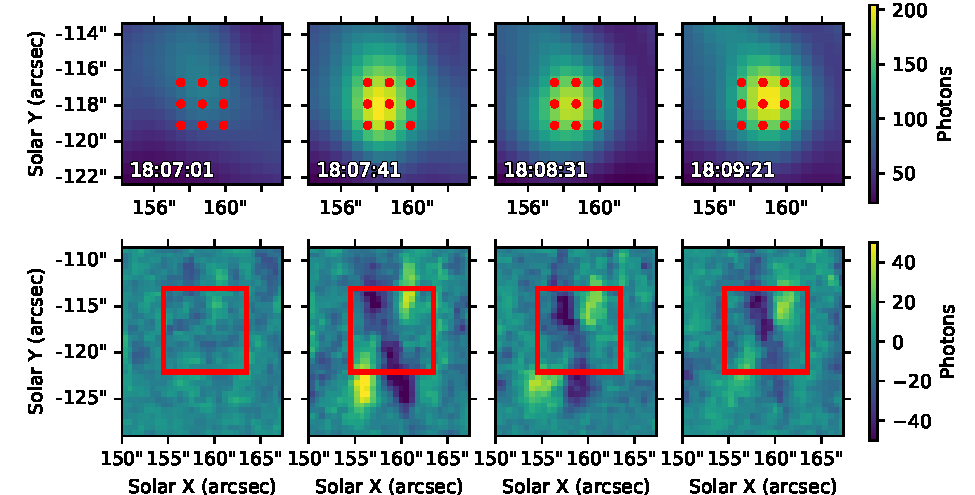
\includegraphics[]{otherx_inverta}};
					\node[inner sep=0pt] (lps) at (0,-10.8)
					{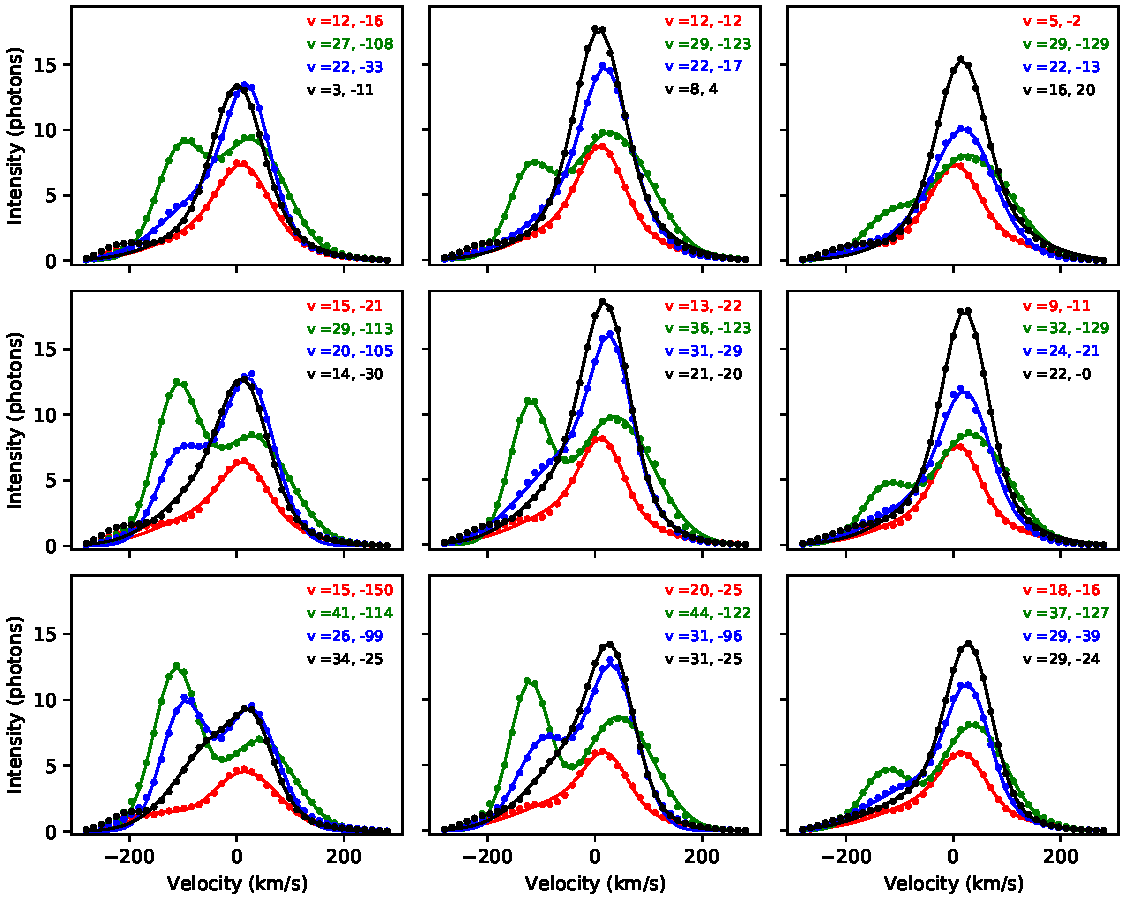
\includegraphics[]{otherx_invertb}};
				\end{tikzpicture}
        	}
%      		\begin{tikzpicture}
%	        	%begin by adding a node for each figure
%	        	\node[inner sep=0pt] (imgs) at (0,0)
%	        	{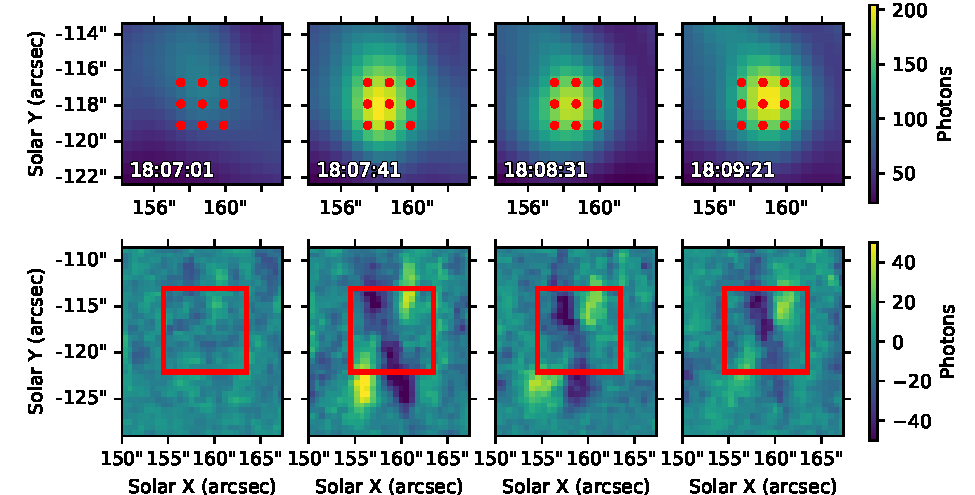
\includegraphics[]{otherx_inverta}};
%	        	\node[inner sep=0pt] (lps) at (0,-10.8)
%	        	{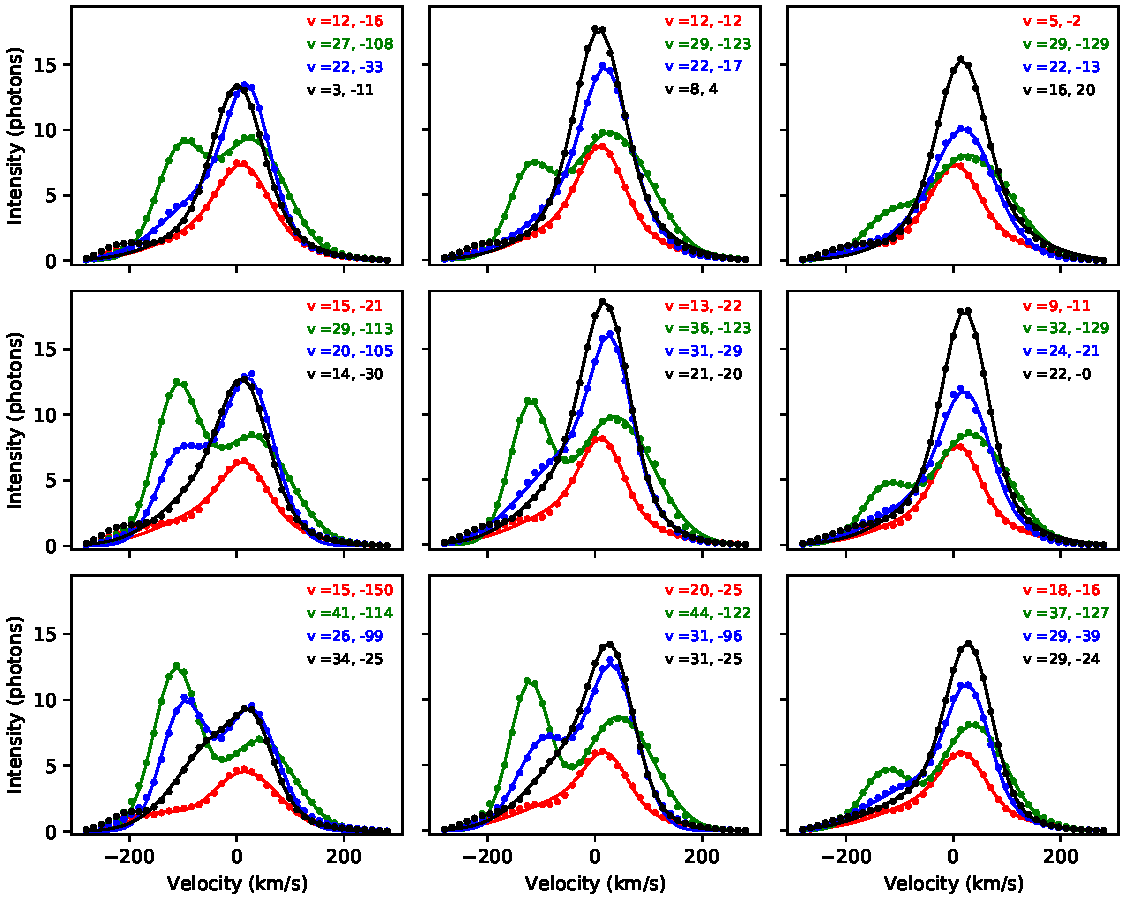
\includegraphics[]{otherx_invertb}};
%        	\end{tikzpicture}
    	\caption{MART inverted results for event d in Figure \ref{fig:l3_dif} presented in the same fashion as Figure \ref{fig:perfect_x_inverted}.}
    	\label{fig:other_x_inverted}
    	\end{figure}
    	
    	In Figures \ref{fig:perfect_x_inverted} and \ref{fig:other_x_inverted}, and their associated animations, we present the MART inversion for two different compact transient events, labeled c and d in Figure \ref{fig:l3_dif}.
    	Both events have an X-shaped presentation, begin and end within the ESIS observing time, and show noticeable temporal evolution in velocity.
		Each figure shows the total \ov \ integrated intensity, obtained by summing the MART inversion along the wavelength dimension, in the top row  at four different times. 
		The second row shows uninverted Channel 2-3 Level 3 difference images at those same times for comparison.
		The FOV of the intensity image from the top row is shown as a red box on the difference image.
		Inverted \ov\ line profiles are plotted in a $3\times 3$ grid, corresponding to the grid of 9 positions marked in red on the intensity images. The red, green, blue, and black curves correspond to the four times indicated in the top row.
		We performed a double Gaussian fit for each line profile in order to more easily pick out the location of each peak in velocity.
		The results of the fit (solid line) is plotted over the MART inverted data (dots).
		The deviation from line center of each Gaussian is recorded in km s$^{-1}$ in the color matching the line profile.
		In the animation, we plot the red and blue components of each fit separately as dashed lines, their sum as a solid line in fuschia, and the MART inverted line profile in  green dots.
		
		Event c, shown in Figure \ref{fig:perfect_x_inverted}, lasts just over 4 minutes and shows significant temporal evolution in the line profile.
		Throughout the event the blue component of the \ov \ line dominates and is centered at $\approx -50$\,km\,s$^{-1}$.
		This blue component persists for the entire duration of the event with % very slight deviations 
		relatively gradual changes in intensity and velocity.
		The red component of the event is bursty in nature, with two small peaks in intensity at 18:07:36 and 18:08:16, and is centered at $\approx$ 120 km s$^{-1}$. 
	    The red and blue components of the line are only occasionally well separated, but the two Gaussian fit consistently follows the inverted line profiles with only small deviations.
		This explosive event is $\approx$ 3 arcseconds in diameter and shows little spatial variation in the line profile across the event.
		
		The explosive event highlighted in Figure \ref{fig:other_x_inverted}, event d, is similar to event c in that is has enhancements in both the red and blue wing of the line profile, but is more complicated in its presentation.
		Event d  begins around 18:07:16 and its intensity has almost completely died away by the last Level 3 image.
		At the beginning of the event a slightly redshifted component dominates the line profile.
		A strong blue component in the line profile centered near -130\,km\,s$^{-1}$ begins to appear 18:07:16 and peaks at 18:08:06. 
		This blue component is brightest in the lower left portion of the event.
		The red component of the line profile peaks at 18:08:56 and is centered near 50 km s$^{-1}$.
		Unlike event c, the blue component of the line is less persistent in time.
		Also, the blue and red components of the event do not occur in the same spatial location.
		This is visible both in the grid of line profiles and the difference images.
		Intensity in the line profiles show the blue component peaking in the lower left, while the red component peaks in the middle to right columns.
		In the difference images, this corresponds to a clear vertical and horizontal separation between the blue $\Lambda$ and the red V. 
		A closer look at the inverted data shows an $\approx$ 1.35 arcsecond spatial separation between centroids of the blue and red component.
	    		   	
        There are two free parameters in our MART algorithm, namely the exponent used in the contrast enhancement filter and the number of times it is applied (Appendix \ref{MART} steps \ref{step:contrast} and \ref{step:smooth}). The inversions in this section were tried with a wide range of these parameters. 
        The Appendix shows the results of tweaking these free parameters for a single timestamp of Event C.
        We find that the results are robust to variation in both parameters. 
        In particular, we consistently find line profiles consistent with a qualitative interpretation of the difference image movies, and measure bulk flows within $\approx\pm$ 15\,km\,s$^{-1}$ ($\approx\pm$ 1\,pixel) for a given exposure. 
    
    	
\section{Discussion/Conclusions and Future Work}
	The ESIS sounding rocket mission, launched September 30, 2019, was successful in capturing spatial and spectral information over is entire \esisfov \ field of view in multiple wavelengths (\hei, \mgxbright, and \ov) at every exposure.
	ESIS is a unique instrument.  
	It is not only a slitless imaging spectrograph, of which there only a handful of examples, it is also a Computed Tomography Imaging Spectrograph (CTIS).  
	To our knowledge, the ESIS and MOSES sounding rocket instruments are the only CTIS instruments ever flown in space to observe the Sun. 
	
	We have processed the  ESIS data into multiple levels such that preliminary scientific work can be done, including a Level 3 data product (Section \ref{sec:level 3}) that allows for taking spatial differences between channels, and early inversion.
	Level 3 difference images in the \ov \ wavelength (Section \ref{sec:dif_images}) reveal a host of small transient brightenings across the field of view with significant line-of-sight Doppler velocity, some in excess of $\pm 100\,$km\,s$^{-1}$.
	They also reveal several larger and more complex events with large velocities, most notably the eruption identified near disk center (event e in Figure \ref{fig:l3_dif}).
	
    During the roughly 5 minutes of ESIS observing time it captured tens of events with supersonic velocities, evolving on 10\,s timescales, over its \esisfov \ field of view.
	Even seemingly simple explosive events evolve fast enough in time, and have significant spatial distributions of intensity and velocity, such that rastering a traditional slit spectrograph would fail to capture the event completely. 
	This, combined with the fact that ESIS can measure many events like this simultaneously, makes it a powerful tool for capturing and diagnosing dynamic events in the solar atmosphere.
	
	We use a Multiplicative Algebraic Reconstruction Technique (MART, Appendix \ref{MART}) to disentangle the combined spatial and spectral information in the four ESIS Level 3 images to find a single spatial-spectral cube $(x,y,\lambda)$, covering just the \ov\ line, for two small transient brightenings (Section \ref{sec:inversions}).
	Our inversions reveal strong red and blue jets with bulk flows in excess of 100\,km s$^{-1}$ that evolve on the timescale of the ESIS cadence, 10 seconds.
	These two events are spatially compact, a few arcseconds, and have lifetimes of a few minutes.
	Despite their compact nature, the red and blue components measured are separate and distinct in both space and time. 
	This is especially noticeable in event d (Figure \ref{fig:l3_dif} and \ref{fig:other_x_inverted}) where the centroids of the blue and red jet are displaced by a little over an arcsecond. 
	
	The bimodal nature of these small brightenings is similar to observations made by \citet{Rust2019} \heii \ using MOSES data, particularly in the case of event d where the separation is visible in the Level 3 data prior to inversion.
	This presentation is different than typical explosive event line profiles typically observed by IRIS in \siiv, where small transient events often show smaller bulk flows, dominant line core emission, non-thermal broadening \citep{Innes2015,Chitta2017}. 
	The bimodal profile and bulk flows exceeding the sound speed ($\approx$ 78\,km\,s$^{-1}$ for O\,\textsc{v} at 225000K) suggest magnetic reconnection occurring in a small region with little to no stationary emitting plasma, most reminiscent of a Petschek type reconnection \citep{Innes1999}.
	Though we hypothesize that both jets originate at a single reconnection site, we admit that it is puzzling that observed fluctuations of the red and blue jets are not temporally correlated, most notably in explosive event d (Figure \ref{fig:other_x_inverted}).
    It is also puzzling that in both events c and d there is a lack of symmetry in velocity between the red and blue jets.
	It may be that the reconnection in these small events is more complex than we imagine and needs to be treated in 3-D; however, it is also possible that, looking in a single spectral line, we are not seeing all of the ejected plasma. 
	Further work with the ESIS data may help to clarify this issue.
	Several of these events were captured in \hei, \mgxbright, and \ov \ simultaneously, putting ESIS in a position to measure the outflows at multiple temperatures. 
	If the event is present in hotter or cooler lines we can also see if the bi-modal nature of these line profiles is unique to \ov \ or persists at lower and higher temperatures.
	Also, IRIS was running small four step coarse rasters near disk center during the hour long ESIS launch window.
	Although none of the events analyzed in this paper were captured by IRIS, a closer look at the IRIS data may reveal small explosive events suitable for direct comparison with ESIS line profiles.
	
	The largest event captured by ESIS (Figure \ref{fig:main_event} and Figure \ref{fig:main_event_aia}) most notably shows a strong red shift at the brightest part of the event (location e1) and a faint string of blue shifted material (location e2) rising above.
	The faint blue shift, combined with the appearance of rising material in the cooler AIA channels, gives the appearance of a small jet or possible mini-filament eruption.
	The brightest part of the event being red shifted also matches the idea that ``jet bright points'', a common feature of smaller jets found at the base of the erupting structure, are the result of a small post-reconnection arcade \citep[see][and references therein]{Sterling2015}.
	The ability of ESIS to capture velocity information across this dynamic event at a 10 second cadence gives us a great advantage when trying understand the underlying physics, and is an exciting opportunity for future study and collaboration.
	Future work on this event will focus on comparing multiple inversion methods, and examining multiple spectral lines in the ESIS passband, to ensure we have the clearest possible picture of the velocity distribution before drawing conclusions.
	
	The next major tasks in the analysis of ESIS data will be to invert the entire spatial-spectral cube, from \spectralline{He}{ii}{584} to \spectralline{O}{v}{630}. 
	A self-consistent inversion will be required to separate out the dimmer \mgxdim, and perhaps even the faint \oiii \ line. This will require a careful characterization of the wavelength-dependent distortion in the images, which is currently underway.
	Future multi-wavelength inversions of the ESIS data will allow for more accurate estimates of the frequency and distribution of explosive events across a large portion of the solar disk and at different heights in the solar atmosphere than have been possible with slit spectrographs.
	It will also allow us to track energy and material moving through multiple layers of the solar atmosphere to form a clearer picture of where and how these reconnection events unfold. 
	
	

	  

